\documentclass[utf8,usehyperref,14pt,final]{G7-32}
\usepackage{graphicx}
\usepackage{textcase}
\graphicspath{{pics/}}
\usepackage[labelsep=endash]{caption}
\captionsetup[table]{singlelinecheck=false} %, margin=5mm}

\usepackage{setspace}
\onehalfspacing
\usepackage[T2A]{fontenc} % кодировка шрифта
\usepackage[russian,english]{babel}
\usepackage{cyrtimes}
%Отступы у страниц
\usepackage{indentfirst}
\renewcommand{\rmdefault}{ftm} % Times New Roman
\setlength{\parindent}{10mm}
\sloppy %переносить длинные слова

\renewcommand{\frontmatter}[1]{
    \clearpage
    \centerline{\MakeTextUppercase{#1}}
    \addcontentsline{toc}{chapter}{#1}
    \vspace{8mm}
}
\renewcommand{\backmatter}[2]{
    \clearpage
    \centerline{\MakeTextUppercase{#1}}
    \centerline{#2}
    \addcontentsline{toc}{chapter}{#1 #2}
    \vspace{8mm}
}
\newcommand\contentsname{\centerline{СОДЕРЖАНИЕ}{~~~}}
\usepackage{listings}

\lstdefinelanguage{JavaScript}{
  keywords={break, case, catch, continue, debugger, default, delete, do, else, finally, for, function, if, in, instanceof, new, return, switch, this, throw, try, typeof, var, void, while, with},
  morecomment=[l]{//},
  morecomment=[s]{/*}{*/},
  morestring=[b]',
  morestring=[b]",
  sensitive=true
}

\lstset{ %
  language=HTML,                 % выбор языка для подсветки (здесь это С)
  basicstyle=\small, % размер и начертание шрифта для подсветки кода
  extendedchars=\true,
  showspaces=false,            % показывать или нет пробелы специальными отступами
  showstringspaces=false,      % показывать или нет пробелы в строках
  showtabs=false,             % показывать или нет табуляцию в строках
  tabsize=2,                 % размер табуляции по умолчанию равен 2 пробелам
  breaklines=true,           % автоматически переносить строки (да\нет)
  breakatwhitespace=false, % переносить строки только если есть пробел
%   frame=single
}
 % Настройки оформления

\begin{document}

\setcounter{page}{2}
% \renewcommand\contentsname{\centerline{СОДЕРЖАНИЕ\vspace{100mm}}{~~~}}
\def\contentsname{СОДЕРЖАНИЕ\vspace{10mm}}
\tableofcontents
\clearpage

На этапе проектирования приложения была проведена декомпозиция на три логические части:

\begin{enumerate}
 \item Построение нового задания для создания исследования.
 \item Отображение списка поставленных исследований.
 \item Вывод подробной информации о проведенном исследовании.
\end{enumerate}

Для каждой части приложения были сверстаны свои шаблоны, описаны модели и закодированы контроллеры.

На этапе построения нового задания клиентское приложение запрашивает у веб-сервиса список доступных алгоритмов для постановки в очередь заданий. Также для каждого алгоритма получается список необходимых параметров. После чего из шаблона формируется форма со списком доступных алгоритмов. При смене алгоритма меняется и набор параметров. После заполнения полей формы, происходит валидация выбранных значений и отправляется запрос на другой веб-сервис. Этот веб-сервис проводит повторную валидацию полученных данных, связывается с менеджером базы данных и перенаправляет запрос в очередь менеджера. Далее сервис возвращает статус, отображающий успех постановки в очередь и идентификатор запроса. Если ответ приходит с ошибкой, то эта ошибка отображается. При успешном статусе, происходит смена представления: отображается список ранее поставленных заданий для проведения исследований.

В другом представлении происходит отображение списка ранее поставленных задач для исследований. Для каждого задания указывается статус готовности. Вся необходимая информация получается с третьего веб-сервиса, который запрашивает у менеджера базы данных список текущих заданий в очереди, список проведенных исследовании и проводимое в данный момент исследование. На основании этих данных по заданному шаблону представления формируется список и выводится пользователю.

Те исследования, что уже были проведены, доступны для подробного изучения. У различных исследований результаты зависят от поставленных алгоритмов и могут различаться. Приложение посылает идентификатор проведенного исследования на веб-сервис и ожидает результат вместе с его описанием. Результат может даже иметь разный вид. Это могут быть массивы точек, по которым необходимо построить график, или же некоторые статистические характеристики, которые ожидал увидеть пользователь. После обработки описания формата происходит заполнение определенного шаблона представления данными результата и выводится пользователю. % Введение

\chapter{Постановка задачи}

В век коммуникационных устройств, социальных сетей и прочих сервисов, сообщение на расстоянии и мгновенный обмен информацией кажутся чем-то само собой разумеющимися. Однако возможность оставаться на связи именно в те моменты, когда коммуникационная инфраструктура оказывается нарушенной, приобретает особое значение. В подобных случаях все более привлекательным вариантом становится создание беспроводной самоорганизующейся (или ad hoc) сети. Такая структура формирует сама себя всякий раз, когда специально запрограммированные устройства связи оказываются в пределах прямого доступа. Каждое из них выполняет в динамической сети функции и передатчика, и приемника, а также, что очень важно, служит ретрансляционным пунктом для всех ближайших приспособлений. Устройства, расстояние между которыми превышает дальность прямой связи, могут поддерживать связь между собой. Таким образом, каждый узел в сети служит и коммуникатором для собственных сообщений, и элементом инфраструктуры для сообщений других узлов.

Когда вы звоните другу по мобильному телефону, в беспроводной связи задействован только каждый из соединяемых телефонов и ближайшая к нему
вышка сотовой связи. Вышки неподвижны и связаны между собой обширной сетью проводов и кабелей. В беспроводных локальных сетях, в частности Wi-Fi, также используются неподвижные антенны и проводные соединения. Такой подход имеет как достоинства, так и недостатки. Однако использование фиксированной инфраструктуры делает эти сети уязвимыми: их работа нарушается в случае отключения электропитания и других сбоев даже при исправности отдельных телефонов и других мобильных устройств в зоне действия сети.

Надежность динамических сетей намного выше. Ad-hoc сети предлагают уникальные преимущества и универсальность для определенных условий и для определенных приложений. Так как нет фиксированной инфраструктуры, базовых станций, то такие сети могут быть созданы и использоваться в любое время и в любом месте. Управление компьютерной сетью усложняется следующими факторами:
\begin{enumerate}
\item Необходимость экономии электроэнергии портативных устройств приводит к значительному снижению радиуса действия приемо-передающих блоков.
\item Радиус действия снижается также за счет естественных и искусственных препятствий, имеющихся на территории.
\item Малый радиус действия приводит к риску потери связанности сети и невозможности оперативной передачи информации между компонентами.
\item На фактор связанности влияют также перемещения узлов сети на местности.
\end{enumerate}

Разработка таких сетей ведется уже больше трех десятилетий, но лишь в последние годы успехи теории сетей привели к созданию первых рабочих крупномасштабных систем. Для того, чтобы подобные сети получили широкое распространение, требуется еще ряд технических прорывов, но на нескольких направлениях успехи уже достигнуты. В качестве основного формального представления такой сети используется геометрический граф. Ребро между двумя узлами сети существует тогда и только тогда, когда расстояние между ними меньше или равно радиусу покрытия этих узлов.

Важным обстоятельством беспроводной самоорганизующейся сети является то, что узлы могут включаться и выключаться из нее в любой момент, что предопределяет случайный характер структуры сети. Именно из этого фактора вытекает необходимость анализа структуры беспроводной сети (геометрического графа) на наличие мостов, путей, маршрутов, компонент связности, циклов и других важных характеристик графа по первому запросу пользователя. При этом результат на запрос должен быть предоставлен как можно быстрее. Для решения этой задачи нами было принято решение о создании программного комплекса вероятностного моделирования ad-hoc сети.

\section{Система вероятностного моделирования ad-hoc сетей}

Для упрощения моделирования и анализа работы системы, а так же для возможности ее расширения было решено придерживаться сервис-ориентированной архитектуры программы, то есть клиент-сервис. Приложение предполагает динамическое подключение библиотек с алгоритмами, что позволит дополнять функционал приложения. Как и во всех приложений такого типа, ресурсоемкие вычисления предполагается проводить на стороне сервера, клиент только оставляет запрос на выполнения определенного алгоритма и ожидает результат.

Программный комплекс состоит из четырех основных частей:
\begin{enumerate}
\item Веб-клиент. Часть, благодаря которой, пользователь сможет подавать запросы на вычисление определенных данных на множестве сетей и получать результаты. Структура клиента генерируется при запуске в зависимости от доступных алгоритмов, что позволяет использовать избавить пользователя от возможных проблем с использованием недоступных на тот момент алгоритмов; 
\item Менеджер заданий. Отвечает за анализ запросов и их дальнейшую обработку, взаимодействует с базой данных и менеджером алгоритмов. Если запрашиваемые данные уже имеются в базе данных, то они сразу отправляются пользователю. В противном случае, данный запрос поступает к менеджеру алгоритмов, и ждет вычисления результатов;
\item Менеджер алгоритмов. Анализирует полученный запрос, после чего запускает необходимый алгоритм на запрашиваемых данных. Время вычислений оптимизируется за счет использования ресурсов, имеющихся на данном компьютере (многопоточность, использование cuda-вычислений);
\item Веб-сервис. Обеспечивает взаимодействие веб-клиента и менеджера заданий, ставя в очередь на выполнения запросы, получаемые от клиента. Так же анализирует информацию о доступных алгоритмах, предоставляемую менеджером алгоритмов, передавая ее веб-клиенту.  
\end{enumerate}
Общая схема проекта представлена на рисунке \ref{structure}.

\begin{figure}[ht]
\center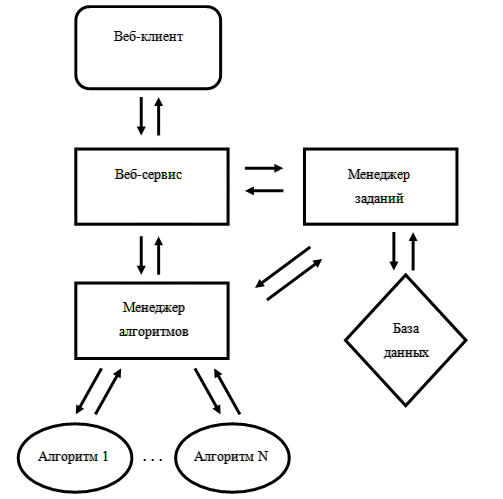
\includegraphics[width=0.8\textwidth]{structure}
\caption{Схема системы вероятностного моделирования ad-hoc сетей}\label{structure}
\end{figure}

Данный проект был дан на реализацию четырем студентам (по количеству частей системного комплекса). Мной было решено реализовывать первую часть описанного программного комплекса – веб-клиент. 


\chapter{Постановка задачи}

В век коммуникационных устройств, социальных сетей и прочих сервисов, сообщение на расстоянии и мгновенный обмен информацией кажутся чем-то само собой разумеющимися. Однако возможность оставаться на связи именно в те моменты, когда коммуникационная инфраструктура оказывается нарушенной, приобретает особое значение. В подобных случаях все более привлекательным вариантом становится создание беспроводной самоорганизующейся (или ad hoc) сети. Такая структура формирует сама себя всякий раз, когда специально запрограммированные устройства связи оказываются в пределах прямого доступа. Каждое из них выполняет в динамической сети функции и передатчика, и приемника, а также, что очень важно, служит ретрансляционным пунктом для всех ближайших приспособлений. Устройства, расстояние между которыми превышает дальность прямой связи, могут поддерживать связь между собой. Таким образом, каждый узел в сети служит и коммуникатором для собственных сообщений, и элементом инфраструктуры для сообщений других узлов.

Когда вы звоните другу по мобильному телефону, в беспроводной связи задействован только каждый из соединяемых телефонов и ближайшая к нему
вышка сотовой связи. Вышки неподвижны и связаны между собой обширной сетью проводов и кабелей. В беспроводных локальных сетях, в частности Wi-Fi, также используются неподвижные антенны и проводные соединения. Такой подход имеет как достоинства, так и недостатки. Однако использование фиксированной инфраструктуры делает эти сети уязвимыми: их работа нарушается в случае отключения электропитания и других сбоев даже при исправности отдельных телефонов и других мобильных устройств в зоне действия сети.

Надежность динамических сетей намного выше. Ad-hoc сети предлагают уникальные преимущества и универсальность для определенных условий и для определенных приложений. Так как нет фиксированной инфраструктуры, базовых станций, то такие сети могут быть созданы и использоваться в любое время и в любом месте. Управление компьютерной сетью усложняется следующими факторами:
\begin{enumerate}
\item Необходимость экономии электроэнергии портативных устройств приводит к значительному снижению радиуса действия приемо-передающих блоков.
\item Радиус действия снижается также за счет естественных и искусственных препятствий, имеющихся на территории.
\item Малый радиус действия приводит к риску потери связанности сети и невозможности оперативной передачи информации между компонентами.
\item На фактор связанности влияют также перемещения узлов сети на местности.
\end{enumerate}

Разработка таких сетей ведется уже больше трех десятилетий, но лишь в последние годы успехи теории сетей привели к созданию первых рабочих крупномасштабных систем. Для того, чтобы подобные сети получили широкое распространение, требуется еще ряд технических прорывов, но на нескольких направлениях успехи уже достигнуты. В качестве основного формального представления такой сети используется геометрический граф. Ребро между двумя узлами сети существует тогда и только тогда, когда расстояние между ними меньше или равно радиусу покрытия этих узлов.

Важным обстоятельством беспроводной самоорганизующейся сети является то, что узлы могут включаться и выключаться из нее в любой момент, что предопределяет случайный характер структуры сети. Именно из этого фактора вытекает необходимость анализа структуры беспроводной сети (геометрического графа) на наличие мостов, путей, маршрутов, компонент связности, циклов и других важных характеристик графа по первому запросу пользователя. При этом результат на запрос должен быть предоставлен как можно быстрее. Для решения этой задачи нами было принято решение о создании программного комплекса вероятностного моделирования ad-hoc сети.

\section{Система вероятностного моделирования ad-hoc сетей}

Для упрощения моделирования и анализа работы системы, а так же для возможности ее расширения было решено придерживаться сервис-ориентированной архитектуры программы, то есть клиент-сервис. Приложение предполагает динамическое подключение библиотек с алгоритмами, что позволит дополнять функционал приложения. Как и во всех приложений такого типа, ресурсоемкие вычисления предполагается проводить на стороне сервера, клиент только оставляет запрос на выполнения определенного алгоритма и ожидает результат.

Программный комплекс состоит из четырех основных частей:
\begin{enumerate}
\item Веб-клиент. Часть, благодаря которой, пользователь сможет подавать запросы на вычисление определенных данных на множестве сетей и получать результаты. Структура клиента генерируется при запуске в зависимости от доступных алгоритмов, что позволяет использовать избавить пользователя от возможных проблем с использованием недоступных на тот момент алгоритмов; 
\item Менеджер заданий. Отвечает за анализ запросов и их дальнейшую обработку, взаимодействует с базой данных и менеджером алгоритмов. Если запрашиваемые данные уже имеются в базе данных, то они сразу отправляются пользователю. В противном случае, данный запрос поступает к менеджеру алгоритмов, и ждет вычисления результатов;
\item Менеджер алгоритмов. Анализирует полученный запрос, после чего запускает необходимый алгоритм на запрашиваемых данных. Время вычислений оптимизируется за счет использования ресурсов, имеющихся на данном компьютере (многопоточность, использование cuda-вычислений);
\item Веб-сервис. Обеспечивает взаимодействие веб-клиента и менеджера заданий, ставя в очередь на выполнения запросы, получаемые от клиента. Так же анализирует информацию о доступных алгоритмах, предоставляемую менеджером алгоритмов, передавая ее веб-клиенту.  
\end{enumerate}
Общая схема проекта представлена на рисунке \ref{structure}.

\begin{figure}[ht]
\center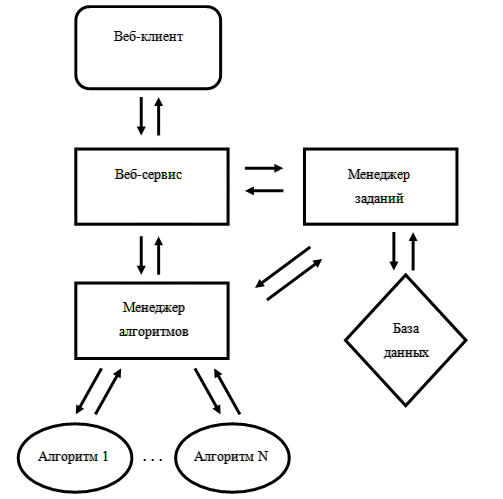
\includegraphics[width=0.8\textwidth]{structure}
\caption{Схема системы вероятностного моделирования ad-hoc сетей}\label{structure}
\end{figure}

Данный проект был дан на реализацию четырем студентам (по количеству частей системного комплекса). Мной было решено реализовывать первую часть описанного программного комплекса – веб-клиент. 


\section{Обзор технологий для веб-разработки}

Развитие современной компьютерной техники и внедрение новейших технологий вызвало появление новых программных продуктов. 
Развиваются не только компьютеры, но и сети. Если еще несколько десятков лет назад Интернет представлял собой небольшую частную сеть, то теперь это гигантская система взаимосвязанных компьютеров, без которой, возможно, мы не сможем представить себе жизнь.
веб-технологии полностью перевернули представление о работе с информацией. Оказалось, что традиционные параметры развития вычислительной техники -- производительность, пропускная способность, емкость запоминающих устройств -- не учитывали главного <<узкого места>> системы -- интерфейса с человеком. И только когда интерфейс между человеком и компьютером был упрощен до естественности восприятия обычным человеком, последовал беспрецедентный взрыв интереса к возможностям вычислительной техники[1].

Веб-приложения представляют собой особый тип программ, построенных по архитектуре <<клиент-сервер>>. Особенность их заключается в том, что само веб-приложение находится и выполняется на сервере -- клиент при этом получает только результаты работы. Работа приложения основывается на получении запросов от пользователя (клиента), их обработке и выдачи результата. Передача запросов и результатов их обработки происходит через Интернет как представлено на рисунке \ref{web}

\begin{figure}[ht]
\center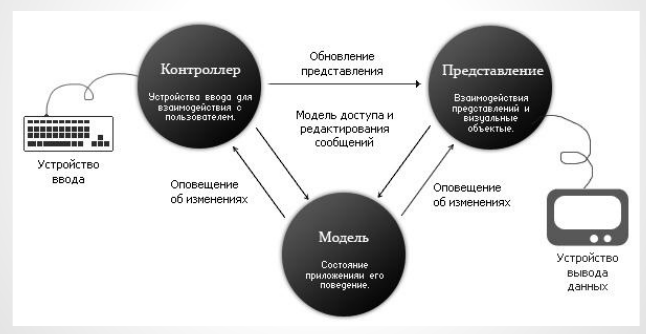
\includegraphics[width=0.9\textwidth]{mvc}
\caption{Архитектура веб-приложения}\label{web}
\end{figure}

За счет наличия исполняемой части, веб-приложения способны выполнять практически те же операции, что и обычные Windows-приложения, с тем лишь ограничением, что код исполняется на сервере, в качестве интерфейса системы выступает браузер, а в качестве среды, посредством которой происходит обмен данными, -- Интернет. К наиболее типичным операциям, выполняемым веб-приложениями, относятся:
\begin{enumerate}
\item прием данных от пользователя и сохранение их на сервере;
\item выполнение различных действий по запросу пользователя: извлечение данных из базы данных (БД), добавление, удаление, изменение данных в БД, проведение сложных вычислений;
\item аутентифицирование пользователя и отображение интерфейса системы, соответствующего данному пользователю;
\item отображение постоянно изменяющейся оперативной информации и т.д.
\end{enumerate}

Современные веб-приложения -- это порталы, предоставляющие услуги. Более четкую иерархию веб-приложений можно посмотреть на рисунке \ref{type_sites}
В настоящее время с точки зрения назначения различают три основных типа порталов:
\begin{enumerate}
\item Публичные, или горизонтальные, порталы (называемые иногда мегапорталами), такие как Rambler. Такие порталы нередко являются результатом развития поисковых систем. Предназначены они для самой широкой аудитории, что отражается на содержании предоставляемой ими информации и услуг. Как правило, эта информация носит общий характер, равно как и предоставляемые услуги (электронная почта, новостные рассылки и так далее).
\item  Вертикальные порталы. Этот вид порталов предназначен для специфических видов рынка. Вертикальные обслуживает аудиторию, пользующуюся услугами этого рынка или работающую на нем. Примерами таких порталов могут служить туристические агентства, предоставляющие услуги по бронированию мест в гостиницах, заказу и доставке билетов, доступу к картам и сведениям об автомобильных маршрутах. Или порталы типа business-to-business, позволяющие своим клиентам реализовывать совместные бизнес-операции (например, выбирать поставщиков и осуществлять закупку товаров, проводить аукционы).
\item Корпоративные порталы предназначены для сотрудников, клиентов и партнеров одного предприятия. Пользователи такого портала получают доступ к предназначенным им сервисам и приложениям в зависимости от их роли и персонального профиля[3].
\end{enumerate}

\begin{figure}[ht]
\center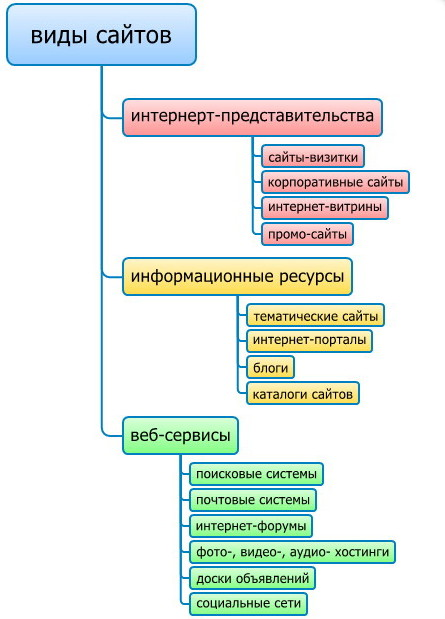
\includegraphics[width=0.5\textwidth]{type_sites}
\caption{Иерархия веб-приложений}\label{type_sites}
\end{figure}

Другие наиболее распространенные веб-приложения:
\begin{enumerate}
\item Региональные Интернет-порталы, универсальные по своему направлению, но ограниченные географией заинтересованных посетителей (e1.ru).
\item Поисковые системы -- это Интернет-порталы, которые предназначены для того, чтобы предоставить их посетителю возможность найти сайты, на которых встречаются заданные слова или целые фразы (yandex.ru, google.ru).
\item Каталог -- это коллекция ссылок на сайты. Зачем же нужны каталоги, если есть поиск? Очень часто мы не знаем точно, что нам нужно, и не можем это сформулировать парой слов (mail.ru).
\item Электронные доски объявлений  являются местом в интернете, где практически любой желающий может оставить информацию ознакомительного, пригласительного или рекламного характера.
\item Форумы -- это специальные сайты или разделы на сайтах, предназначенные для того, чтобы посетители, оставляя свои сообщения, обменивались мнениями, задавали вопросы в поисках ответов.
\item Чаты -- являются еще одним местом для общения в Интернет, только его назначение не обмен мнениями на какую-то тему, а просто времяпрепровождение.
\item Интернет-магазины и аукционы[3].
\end{enumerate}


\section {Серверная часть}

На стороне сервера веб-приложение выполняется специальным программным обеспечением (веб-сервером), который и принимает запросы клиентов, обрабатывает их, формирует ответ в виде страницы, описанной на языке HTML, и передает его клиенту.

В процессе обработки запроса пользователя веб-приложение компонует ответ на основе исполнения программного кода, работающего на стороне сервера, веб-формы, страницы HTML, другого содержимого, включая графические файлы. В результате, как уже было сказано, формируется HTML-страница, которая и отправляется клиенту. Получается, что результат работы веб-приложения идентичен результату запроса к традиционному веб-сайту, однако, в отличие от него, веб-приложение генерирует HTML-код в зависимости от запроса пользователя, а не просто передает его клиенту в том виде, в котором этот код хранится в файле на стороне сервера. То есть веб-приложение динамически формирует ответ с помощью исполняемого кода -- так называемой исполняемой части.

{\itshape PHP } -- скриптовый язык. В первую очередь PHP используется для создания скриптов, работающих на стороне сервера, для этого его, собственно, и придумали. PHP способен решать те же задачи, что и любые другие CGI-скрипты, в том числе обрабатывать данные html-форм, динамически генерировать html страницы и тому подобное. Но есть и другие области, где может использоваться PHP.
Вторая область – это создание скриптов, выполняющихся в командной строке. То есть с помощью PHP можно создавать такие скрипты, которые будут исполняться, вне зависимости от веб-сервера и браузера, на конкретной машине.
И последняя область – это создание GUI-приложений (графических интерфейсов), выполняющихся на стороне клиента\cite{php}.

{\itshape VBScript} -- язык создания сценариев VBScript разработан фирмой Microsoft, является подмножеством достаточно распространенного в среде программистов языка Visual Basic разработки прикладных программ Windows-приложений. Как и его родитель, язык VBScript достаточно прост и легок в изучении.
Преимуществом его применения для создания сценариев является возможность использования, с небольшими корректировками, ранее написанных процедур на языках Visual Basic и Visual Basic for Application.
Функциональные возможности сценариев, написанных на VBScript, ничем не отличаются от возможностей сценариев JavaScript: динамические создание документа или его частей, перехват и обработка событий и так далее.
VBScript используется для написания сценариев клиента (в этом случае браузер должен иметь встроенный интерпретатор этого языка), а также для написания сценариев на сервере (в этом случае сервер должен поддерживать язык VBScript).
Для создания сценариев клиента используется набор объектов, аналогичный набору JavaScript. Объекты клиента и сервера отличаются друг от друга, но существует общая часть (ядро) объектов, используемых при разработке как сценариев клиент, так и сценариев сервера\cite{VBS}.

{\itshape Perl} -- скриптовый язык. Наиболее широко Perl используется для разработки инструментов системного администрирования, однако в последнее время он получил огромную популярность в области разработки Интернет-приложений: CGI-сценариев, систем автоматической обработки электронной почты и поддержки узлов Web\cite{perl}.
Вот некоторые примеры задач, которые можно решать с помощью Perl:
\begin{enumerate}
\item проверка пользователей Windows NT на несоответствие их статуса и возможностей;
\item управление NT-сервисами из командной строки и дистанционно с локальной машины получение статистических данных на отдельной машине;
\item может работать и с протоколом FTP;
\item системная поддержка UNIX и Windows.
\end{enumerate}

\section {Клиентская часть}

Отображением результатов запросов, а также приемом данных от клиента и их передачей на сервер обычно занимается специальное приложение -- браузер. Как известно, одной из функций браузера является отображение данных, полученных из Интернета, в виде страницы, описанной на языке HTML, следовательно, результат, передаваемый сервером клиенту, должен быть представлен на этом языке.
Рассмотрим основные инструменты, с помощью которых можно создать любой веб-сайт.

{\itshape HTML } --  язык разметки гипертекста (Hypertext Markup Language)  -- это компьютерный язык, лежащий в основе World Wide Web (Всемирной Паутины). Благодаря языку HTML любой текст можно разметить, преобразовав его в гипертекст с последующей публикацией в веб.
Язык HTML имеет собственный набор символов, с помощью которых веб-браузеры отображают страницу. Эти символы, называемые дескрипторами, включают в себя элементы, необходимые для создания гиперссылок.
Одной из отличительных особенностей HTML-документов является то, что сам документ содержит только текст, а все остальные объекты встраиваются в документ в момент его отображения Браузером с помощью специальных тэгов и хранятся отдельно. При сохранении HTML-файла в месте размещения документа создается папка, в которую помещаются сопутствующие ему графические элементы оформления\cite{php}.

Веб-сайт должен быть не только функциональным, но и привлекательным. Для того чтобы приукрасить обычную HTML-страницу, наполненную текстом, понадобиться инструмент {\itshape Cascading Style Sheets } -- формальный язык описания внешнего вида документа, написанного с помощью языка разметки.  CSS используется создателями веб-страниц для задания цветов, шрифтов, расположения отдельных блоков и других аспектов представления внешнего вида этих веб-страниц. Основной целью разработки CSS являлось разделение описания логической структуры веб-страницы (которое производится с помощью HTML или других языков разметки) от описания внешнего вида этой веб-страницы (которое теперь производится с помощью формального языка CSS). Такое разделение может увеличить доступность документа, предоставить большую гибкость и возможность управления его представлением, а также уменьшить сложность и повторяемость в структурном содержимом. Кроме того, CSS позволяет представлять один и тот же документ в различных стилях или методах вывода\cite{php}.

Но язык разметки не обладает логикой, не умеет обрабатывать данные -- только отображать. Для того чтобы наделить клиентскую часть функционалом и создать интерактивный HTML-документ, используют язык программирования {\itshape JavaScript }. Это прототипно-ориентированный сценарный язык разработки встраиваемых приложений, выполняющихся как на стороне клиента, так и на стороне сервера\cite{php}.
Основные области применения JavaScript делятся на следующие категории:
\begin{enumerate}
\item динамическое создание документа с помощью сценария;
\item оперативная проверка достоверности заполняемых пользователем полей форм HTML до передачи их на сервер;
\item создание динамических HTML-страниц совместно с каскадными таблицами стилей и объектной моделью документа;
\item взаимодействие с пользователем при решении <<локальных>> задач, решаемых приложением JavaScript, встроенном в HTML-страницу.
\end{enumerate}

Частая перезагрузка страницы снижает производительность и удобство работы с веб-сайтом. Для того чтобы на каждый запрос сервер не выдавал новую страницу, а отсылал лишь те данные, которые нужны клиенту, в HTML из них прямо в браузере формирует движок Ajax.
{\itshape Ajax } расшифровывается как Asynchronous Javascript And XML и технологией в строгом смысле слова не является. Он определяет, какие запросы можно обработать <<на месте>>, а за какими необходимо обращаться на сервер. Асинхронность проявляется в том, что далеко не каждый клик пользователя доходит до сервера, причем обратное тоже справедливо -- далеко не каждая реакция сервера обусловлена запросом пользователя. Большую часть запросов формирует движок Ajax, причем его можно написать так, что он будет загружать информацию, предугадывая действия пользователя\cite{php}.
Где стоит использовать Ajax:
\begin{enumerate}
\item Формы. Если асинхронно передавать данные, страница не перезагружается, что заметное ускоряет работу.
\item Навигация в виде <<дерева>>. Такая навигация не является удобной и лучше использовать простую топологию, но если уж до этого дошло, лучше использовать Ajax.
\item Голосования. Пользователю будет приятней оставить свой голос за несколько секунд, чем за 30-40.
\item Фильтры. Часто на сайтах делают сортировку по дате, по имени. Ajax это будет значительно удобнее.
\end{enumerate}

 
{\itshape jQuery}-- библиотека JavaScript, фокусирующаяся на взаимодействии JavaScript и HTML. Библиотека jQuery помогает легко получать доступ к любому элементу DOM, обращаться к атрибутам и содержимому элементов DOM, манипулировать ими. Также библиотека jQuery предоставляет удобный API для работы с Ajax. jQuery обладает широким спектром возможностей, главными из которых являются визуальные эффекты, Ajax-дополнения и JavaScript-плагины\cite{php}.


\clearpage

\section {Обзор инструментов для реализации веб-приложения}

\subsection{Single Page Application}

Основной задачей данного проекта является реализация веб-приложения, взаимодействующее с веб-сервером по протоколу SOAP. Результатом проекта должно получится приложение, которое сможет быстро и мгновенно реализовывать функциональные операции. В настоящее время в сфере веб разработки наряду с многостраничными сайтами (Multi-page Application, MPA) широкое распространение получили и одностраничные приложения (Single-page Application, SPA), формирование контента которых происходит динамически на стороне клиента. В связи с этим было решено реализовывать одностраничное приложение. На рисунках  \ref{mpa} и  \ref{spa} представлена схема работы многостраничного и одностраничного сайта соответственно.

\begin{figure}[ht]
\center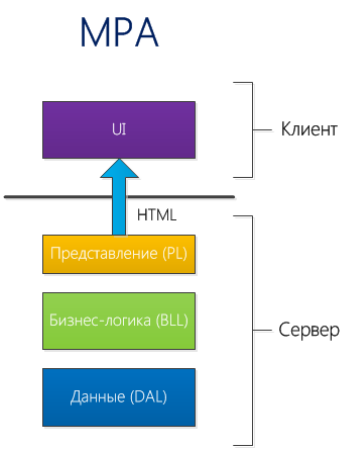
\includegraphics[width=0.4\textwidth]{mpa}
\caption{Архитектура Multi-page Application}\label{mpa}
\end{figure}

\begin{figure}[ht]
\center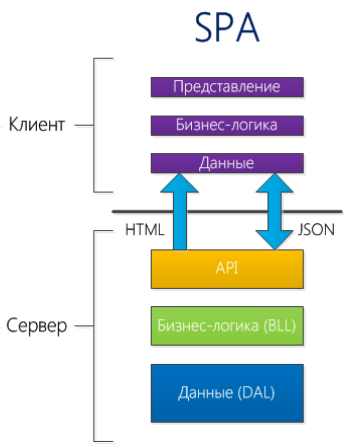
\includegraphics[width=0.4\textwidth]{spa}
\caption{Архитектура Single Page Application}\label{spa}
\end{figure}

Single Page Application -- это веб-приложение, размещенное на одной странице. Применяя такую технологию, можно создать сайт,  который будет представлять собой одну html-страницу, интерактивность которой обеспечивается скриптами. Работа такого веб-сайт максимально полностью перенесена на сторону клиента. Сайт <<общается>> с сервером только чистыми данными, без загрузки html-контента.
 
Для того чтобы написать одностраничное приложение необходимо придерживаться определенных правил:
\begin{enumerate}
\item Все сущности приложения основаны на моделях и объектах. Внутри объектов инкапсулирована работа с DOM-элементами страницы.
\item Насколько позволяет структура хранит HTML шаблоны в скриптах
\item При любые изменения на странице динамически изменяют url.
\item Прямая загрузка любого url должна отобразить соответствующую страницу с данными.
\item Обработчик события History back, что соответствует кнопки назад в браузере, должен выполняться корректно и возвращать страницу в предыдущее состояние.
\item Кеширование моделей данных на стороне клиента.
\end{enumerate}

Если учитывать эти основные правила, в результате получится эффективное, быстрое и полнофункциональное одностраничное веб-приложение.   Но как и любой продукт, приложение обладает рядом преимуществ и недостатков. Рассмотрим плюсы и минусы данного подхода и почему SPA все равно остается популярным.

К преимуществам SPA можно отнести следующее:
\begin{enumerate}
\item Работа на большом количестве устройств. Приложения на SPA отлично работают на устройствах как стационарных, так и мобильных. Персональные компьютеры, планшеты, смартфоны могут беспрепятственно работать с сайтами построенных по принципу SPA. Создав одно приложение, мы получим гораздо большую аудиторию пользователей нежели при использовании стандартного подхода.
\item  Богатый пользовательский интерфейс. Так как веб-страница одна, построить функциональный и приятный пользовательский интерфейс гораздо проще. Не так затруднительно хранить информацию о сеансе, управлять состояниями представлений и управлять анимацией.
\item Отсутствие загрузки одного и того же контента снова и снова. Если сайт использует шаблон, то вместе с основным содержанием какой-либо страницы посетитель сайта обязательно загружает разметку шаблона. Конечно, кеширование данных на данном этапе развития в веб-программировании достигло высоких результатов, но если нечего кешировать, то время  и ресурсы на это не тратятся.
\end{enumerate}

Самым главным неудобством при разработке SPA -- это работа с языком программирования JavaScript. JavaScript изначально позиционировался как простой язык программирования с Java-подобным синтаксисом. Но  JavaScript не обладает статической типизацией, его объектная модель не является привычной для многих разработчиков. Отладка кода представляет собой трудный процесс. Кроме того, различные интернет-обозреватели могут по-разному интерпретировать JavaScript-код. Поэтому разработка требуемого приложения с использованием исключительно языка JavaScript является довольно трудоемким процессом. Чтобы как-то исправить несовместимость с некоторым браузерами, приходится писать отдельный код для различных клиентов. Таким образом, размер кода возрастает, а функциональность нет. В итоге приходится основную часть времени тратить на обработку особенностей выполнения кода различными движками, а не на реализацию продукта. Частично последнюю проблему можно решить использованием специальных библиотек, примеру, библиотека jQuery.  


\subsection {JavaScript-фреймворки}

На смену библиотекам вроде jQuery в мир JavaScript приходят фреймворки, реализующие функциональную схему Model-view-controller. 

Model-view-controller (MVC) -- схема использования нескольких шаблонов проектирования, с помощью которых модель приложения, пользовательский интерфейс и взаимодействие с пользователем разделены на три отдельных компонента таким образом, чтобы модификация одного из компонентов оказывала минимальное воздействие на остальные. Архитектура работы MVC представлена на рисунке \ref{mvc}

\begin{figure}[ht]

\center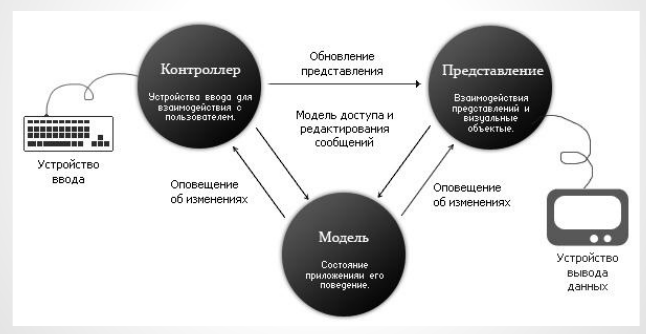
\includegraphics[width=0.7\textwidth]{mvc}

\caption{Схема Model-view-controller}\label{mvc}

\end{figure}

Концепция MVC позволяет разделить данные, представление и обработку действий пользователя на три отдельных компонента:
\begin{enumerate}
\item Модель (англ. Model). Модель предоставляет знания: данные и методы работы с этими данными, реагирует на запросы, изменяя свое состояние. Не содержит информации, как эти знания можно визуализировать.
\item Представление, вид (англ. View). Отвечает за отображение информации (визуализацию). Часто в качестве представления выступает форма (окно) с графическими элементами.
\item Контроллер (англ. Controller). Обеспечивает связь между пользователем и системой: контролирует ввод данных пользователем и использует модель и представление для реализации необходимой реакции.
\end{enumerate}

Важно отметить, что как {\itshape представление}, так и {\itshape контроллер} зависят от {\itshape модели}. Однако модель не зависит ни от представления, ни от контроллера. Тем самым достигается назначение такого разделения: оно позволяет строить модель независимо от визуального представления, а также создавать несколько различных представлений для одной модели.


Преимущества фреймворков видны невооруженным глазом. Один из самых существенных является избавление от рутинного кода, который тянется от проекта к проекту. Фреймворк предоставляет разработчикам каркас будущего приложения и решение задач, встречающихся в большинстве проектов. Например, программисту не нужно думать, как принять данные от клиента и передать их на сервер, т.к. все необходимое скорей всего реализовано авторами фреймворка. Вместо этого разработчику предлагается сосредоточиться функционалом собственного приложения.

Другим немаловажным плюсом всех фреймворков является стандартизация кодирования. Если разработчик решается применять готовый каркас в своем проекте, то он должен быть готовым следовать его заповедям. Это значит, что ему нужно не полениться - один раз ознакомиться с правилами и быть спокойным, что в последствие код без проблем может дорабатываться другими разработчиками. 

Очень часто многие разработчики задают вопрос -  Чем один Javascript фреймворк лучше другого? На этот вопрос трудно ответить, ведь каждый фреймворк обладает определенным набором инструментов и имеет свой круг задач, с которыми он успешно справляется. Выбор JavaScript MVC фреймворка — тяжелая работа. Нужно учесть много факторов, и число вариантов выбора может быть огромно. 


Для создание приложения на основе SPA необходимо отобрать несколько фреймворков, чей функционал справится с поставленной задачей, рассмотреть сильные и слабые стороны каждого и выбрать подходящий вариант.

\subsection {Angular}

AngularJS --- MVW-фреймворк для разработки качественных клиентских веб-приложений на JavaScript. Он создан и поддерживается в Google и предлагает взглянуть на будущее веба, на то, какие новые возможности и стандарты он готовит для нас. MVW означает Model-View-Whatever (модель--вид--что-угодно), то есть гибкость в выборе шаблонов проектирования при разработке приложений. Мы можем выбрать модели MVC (Model--View--Controller) или MVVM (Model--View--View--Model) [4].

AngularJS является основой, которая связывает HTML-код, который генерируется для просмотра страницы в окне браузера с JavaScript объектами. Когда изменяется один из объектов, автоматически обновляется и генерируемая страница. Верно и обратное --- модели связаны с контентом страницы. Когда изменяется контент, это вызывает изменения и в коде сайта. Это называется двусторонней связью данных, схематично представленной на рисунке \ref{dual}.

\begin{figure}[ht]
\center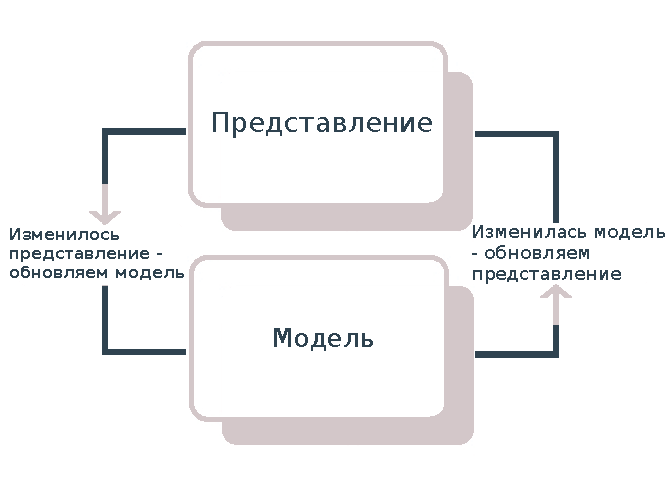
\includegraphics[width=0.9\textwidth]{dual}
\caption{Схема двусторонней привязки данных}\label{dual}
\end{figure}

AngularJS связывает коды в единую систему, и разработчику не нужно больше обновлять HTML вручную или инспектировать элементы, как в случае, если приходится использовать JQuery.
Инъекция зависимостей – шаблон разработки программ, который определяет, как компоненты связываются со своими зависимостями. Инъекция — это передача зависимости к зависимому Объекту, и эти зависимости часто называют Сервисами.

В AngularJS используются аргументы функции для объявления нужных зависимостей. Если мы забудем передать зависимость, но сошлемся на нее там, где она нужна нам, Сервис будет не определен и в результате произойдет ошибка компиляции внутри Angular. Однако, Angular выбрасывает свои ошибки, и они очень просты в отладке.

Одно из основных понятий в программировании – область видимости. В Angular область видимости – это один из главных объектов, который делает возможным циклы двусторонней связи данных и сохраняет состояние приложения. \textdollar scope --- объект, который не только имеет доступ к данным и значениям, но и предоставляет эти данные в DOM, когда Angular рендерит наше приложение.

\textdollar scope – это автоматический мост между JavaScript и DOM, хранящий синхронизированные данные[4]. Это позволяет проще работать с шаблонами, когда мы используем при этом синтаксис HTML, а Angular рендерит соответствующие значения \textdollar scope. Это создает связь между JavaScript и DOM. Таким образом, \textdollar scope играет роль ViewModel.

Контроллер позволяет взаимодействовать Виду и Модели. Это то место, где логика презентации синхронизирует интерфейс с моделью. Цель Контроллера – приводить в действие изменения в Модели и Виде. В Контроллере Angular сводит вместе бизнес-логику и логику презентации. Контроллер принимает два аргумента – имя, по которому на него можно ссылаться, и функцию обратного вызова. При этом на самом деле это будет функция, описывающая тело Контроллера.

Цель Контроллера – интерпретировать бизнес-логику модели и преобразовывать ее в формат презентации. В AngularJS это можно делать по-разному, в зависимости от того, какие мы получаем данные.
Контроллер общается с Сервисом, и передает данные в том же, или измененном формате в наш Вид через объект \textdollar scope. Когда Вид обновлен, логика Контроллера также обновляется, и ее можно передавать обратно на сервер через Сервис.
HTML отлично подходит для описания статичных документов, но теряет свою эффективность при попытке описать динамические виды в веб-приложениях. AngularJS позволяет расширить синтаксис HTML. В результате код получается выразительным, читаемым, и легко поддерживается.

\subsection {BackBone}

Приложения на Backbone не придерживаются строгой архитектуры. Основная идея, которую несет документация: используйте инструменты этого фреймворка так, как вам хочется. Благодаря такому подходу Backbone хорош для абсолютно разных задач, и на нем очень просто начать писать приложения. Однако с другой стороны, это приводит к тому, что новички совершают ошибки в самом начале работы с ним. 

Работая с Backbone, данные представляются как Модели (Models), которые могут быть созданы, провалидированы, удалены, и сохранены на сервере. Всякий раз, когда в интерфейсе изменяется атрибуты модели, модель вызывает событие "change"; все Представления (Views), которые отображают состояние модели, могут быть уведомлены об изменении атрибутов модели, с тем чтобы они могли отреагировать соответствующим образом — например, перерисовать себя с учетом новых данных. При изменении модели представление просто обновит себя самостоятельно.

Рассмотрим поподробней сущности Backbone, их предназначение и минимальную реализацию:
\begin{enumerate}
\item Backbone.Model; Model  -- это единица данных. Отвечает за получение, отправку, хранение, валидацию и прочие манипуляции с данными какой-то сущности. Простая реализация такой единицы данных представлена на рисунке \ref{modal}.

\item Backbone.Collection; Collection -- это упорядоченный набор  моделей. Отвечает за получение и отправку данных какой-то сущности, а так же манипуляции с моделями (создание, обновление, удаление). Работает только с моделями определенного типа. Простая реализация такого списка представлена на рисунке \ref{collection}.

\item Backbone.View; View -- это представление модели или коллекций, отвечает за реализацию интерфейса. Отвечает за рендеринг модели или коллекции, работу с шаблонами, обработку событий и другое. Простая реализация представлена на рисунке \ref{view}.

\item Backbone.Router; Router предоставляет методы для маршрутизации на стороне клиента, а также связывания этих действий с событиями. Простая реализация таких методов представлена на рисунке \ref{router}.

\end{enumerate}

\begin{figure}[ht]
\center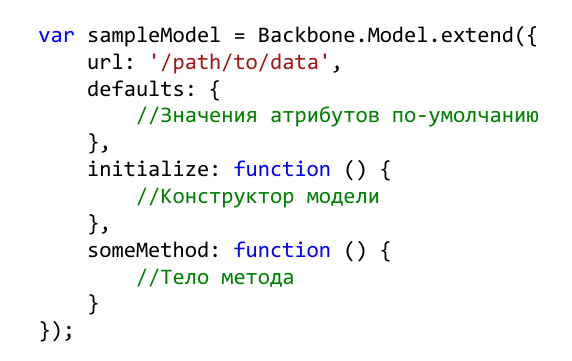
\includegraphics[width=0.75\textwidth]{model}
\caption{Backbone.Model}\label{modal}
\end{figure}

\begin{figure}[ht]
\center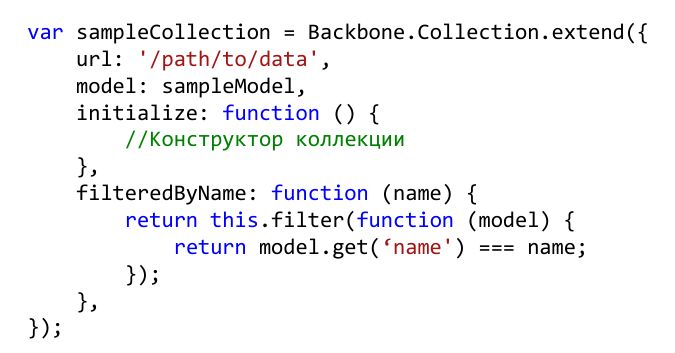
\includegraphics[width=0.75\textwidth]{collection}
\caption{Backbone.Collection}\label{collection}
\end{figure}


\begin{figure}[ht]
\center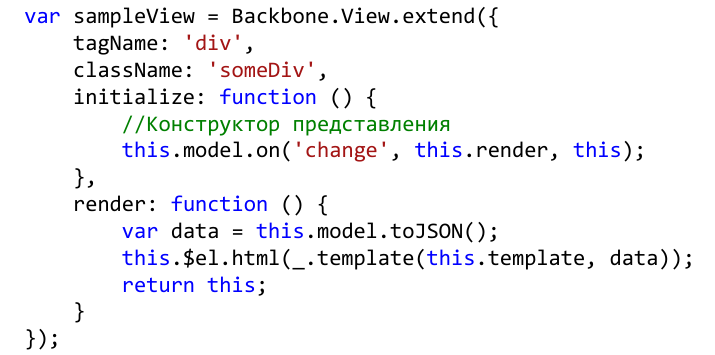
\includegraphics[width=0.75\textwidth]{view}
\caption{Backbone.View}\label{view}
\end{figure}

\begin{figure}[ht]
\center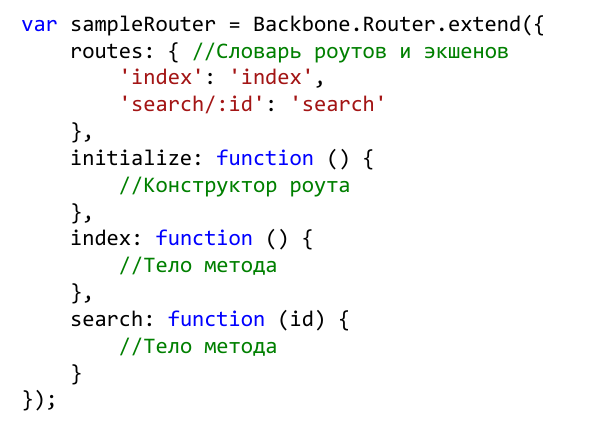
\includegraphics[width=0.75\textwidth]{router}
\caption{Backbone.Router}\label{router}
\end{figure}

\subsection {Сравнение Angular и BackBone}

Перед тем как реализовывать приложение, были тщательно изучены и опробованы оба фреймворка. Были выбраны характеристики, которые являются важными при реализации приложения, и на основе полученных данных произвели сравнение фреймворков. характеристики для сравнения:
\begin {enumerate}
\item Порог входа и документация
\item Продуктивность разработки
\item Набор функций
\item Размер 
\item Защита от утечки памяти 
\end {enumerate}

{\itshape Порог входа и документация}

Angular легко позволяет делать сложные вещи такие, как двунаправленная синхронизация. Но после освоения базовых знаний, порог обучения становится выше: открывается сложная структура с большим количеством особенностей. Чтение документации затруднено из-за специфического жаргона и малого количества примеров.

Backbone — довольно прост в освоении. Но после длительного использования вы можете обнаружить, что не хватает понимания того, как лучше структурировать код. Чтобы исправить сложившуюся ситуацию необходимо просмотреть или прочитать несколько учебников. 

{\itshape Продуктивность разработки}

Разработка с помощью Angular будет достаточно быстрой и эффективной, после того, как изучить его основные функции и принцип работы.

Backbone требует написания очень большого объема шаблонного кода. Что оказывается прямой угрозой производительности труда и является неэффективным.

{\itshape Набор функций}

Среди основного набора функций, которым обладает схема MVC является:
\begin{enumerate}
\item Реализация паттерна <<Наблюдатель>>: объекты, изменения которых отслеживаются.
\item  Наличие автоматически изменяемых представлений
\item Представления (визуализация шаблонов), включающие другие представления.
\item Показ представлений по некоторым условиям.
\item Использование автоматически изменяемых представлений, когда наблюдаемый объект изменяется.
\end{enumerate}

Angular полный набор перечисленных функций.

Backbone, в свою очередь, иметь только реализацию паттерна <<Наблюдатель>>

{\itshape Размер и зависимости} 

Является важным фактором для мобильной разработки.

Angular имеет размер в 80 килобайт, однако это единственный фреймворк, не требующий дополнительных библиотек.

Backbone считается самым маленький фреймворк, но требует как минимум две библиотеки, что увеличивает размер фреймворка до 61 килобайта.

{\itshape Защита от утечки памяти} 

Так же является важным фактором для длительно открытых одностраничных приложений.

С фреймворком Angular можно эффективно решать проблему с утечкой памяти, даже не обладая огромным опытом в разработке.

Что нельзя сказать о фреймворке Backbone. При недостаточных знаний эта проблема окажется глобальной.

\subsection{Apache Cordova}
На сегодняшний день люди везде используют мобильные устройства для самых различных потребностей. Будь то фотографирование и размещения снимков в социальных сетях, поиска местоположения ресторана или просмотра заголовков новостей. Мобильные устройства имеют множество форм и стилей. Мобильные телефоны работают на разных операционных системах, таких как Apple iOS, Google Android и Research In Motion Blackberry. Некоторые имеют большие экраны, физические клавиатуры и работают в сетях 3G, 4G или WiFi. Мобильные телефоны могут также иметь датчики ускорения, местоположения и даже платежей. Некоторые из этих устройств - даже не телефоны; это планшеты с более крупными экранами и сетевым подключением только для обмена данными.

Несмотря на различия, мобильные устройства похожи друг на друга тем, что все они исполняют мобильные приложения. Мобильные приложения можно разделить на три типа: встроенные, веб-приложения и гибридные.

Установленные на устройство встроенные приложения представляют собой бинарные исполняемые программы, созданные с использованием соответствующего  SDK  и  распространяемые  через  хранилища приложений. SDK существуют для каждой мобильной операционной системы и, конечно же, различаются между собой.

В отличие от встроенных веб-приложения загружаются в мобильный веб-браузер, их код пишется с использованием веб-технологий (HTML, JavaScript и CSS), не зависящих от операционной системы устройства. Нет необходимости изучать различные языки программирования для каждого устройства. HTML и JavaScript знакомы веб-разработчикам по созданию веб-страниц для настольных браузеров. В большинстве случаев мобильные веб-браузеры могут визуализировать те же самые веб-страницы, но веб-сайты часто предоставляют мобильные версии с меньшим объемом информации и более быстрой загрузкой (из-за меньшего размера экрана и более медленной сети).

Для запуска веб-приложения пользователь вводит URL-адрес в мобильный веб-браузер. После этого загружается веб-страница, являющаяся точкой входа в веб-приложение. Веб-приложения не распространяются через хранилище приложений; они являются обычными ссылками, которые можно включить в другие веб-страницы.

Гибридные приложения, как и веб-приложения, программируются с использованием веб-технологий, но пакетируются как встроенные приложения. Гибридное приложение можно написать сразу для нескольких мобильных операционных систем с использованием языка программирования, знакомого многим разработчикам. Поскольку гибридное приложение на самом деле является встроенным, вы получаете доступ к функциям устройства из JavaScript, что пока недоступно для веб-приложений.

Гибридные приложения можно распространять и устанавливать через хранилища приложений, подобно встроенным. Apache Cordova позволяет создавать универсальные мобильные приложения, работающие на различных мобильных платформах, с использованием стандартных веб-технологий (HTML5, CSS3 и JavaScript), что отображено на рисунке \ref{cordova}.

\begin{figure}[ht]
\center
\includegraphics[width=0.9\textwidth]{cordova}
\caption{Apache Cordova}\label{cordova}
\end{figure}

Использование Apache Cordova в качестве базового фреймворка, позволяет создавать приложения, функционирующие на широком спектре мобильных платформ, включая Tizen, webOS, Android, iOS, Blackberry, Samsung Bada и Windows Phone\cite{cordova}.

Cordova предоставляет среду для хостинга контента HTML5/JavaScript внутри тонкой <<родной>> оболочки. Для ОС на каждой платформе смартфонов она использует родной элемент управления <<браузер>> для рендеринга контента создаваемого приложения, причем ресурсы приложения упаковываются в дистрибутив.

Cordova также предоставляет набор стандартных API для доступа к функциям, общим для всех смартфонов. К некоторым из этих функций относятся:
\begin{enumerate}
\item События жизненного цикла приложения.
\item Хранилище (локальное хранилище и базы данных HTML5).
\item Контакты.
\item Камера.
\item Геопозиционирование.
\item Акселерометр.
\end{enumerate}
Каждая из этих функций предоставляется как JavaScript API, который используется из кода на JavaScript. Cordova берет на себя всю черновую работу, связанную с предоставлением необходимой родной реализации, и тем самым гарантирует, что программист будет иметь дело с одинаковыми JavaScript API независимо от ОС смартфона, на котором выполняется код создаваемого приложения. 



\chapter{Выполнение поставленной задачи}

На этапе проектирования приложения была проведена декомпозиция на три логические части:

\begin{enumerate}
 \item Построение нового задания для создания исследования.
 \item Отображение списка поставленных исследований.
 \item Вывод подробной информации о проведенном исследовании.
\end{enumerate}

Для каждой части приложения были сверстаны свои шаблоны, описаны модели и закодированы контроллеры.

На этапе построения нового задания клиентское приложение запрашивает у веб-сервиса список доступных алгоритмов для постановки в очередь заданий. Также для каждого алгоритма получается список необходимых параметров. После чего из шаблона формируется форма со списком доступных алгоритмов. При смене алгоритма меняется и набор параметров. После заполнения полей формы, происходит валидация выбранных значений и отправляется запрос на другой веб-сервис. Этот веб-сервис проводит повторную валидацию полученных данных, связывается с менеджером базы данных и перенаправляет запрос в очередь менеджера. Далее сервис возвращает статус, отображающий успех постановки в очередь и идентификатор запроса. Если ответ приходит с ошибкой, то эта ошибка отображается. При успешном статусе, происходит смена представления: отображается список ранее поставленных заданий для проведения исследований.

В другом представлении происходит отображение списка ранее поставленных задач для исследований. Для каждого задания указывается статус готовности. Вся необходимая информация получается с третьего веб-сервиса, который запрашивает у менеджера базы данных список текущих заданий в очереди, список проведенных исследовании и проводимое в данный момент исследование. На основании этих данных по заданному шаблону представления формируется список и выводится пользователю.

Те исследования, что уже были проведены, доступны для подробного изучения. У различных исследований результаты зависят от поставленных алгоритмов и могут различаться. Приложение посылает идентификатор проведенного исследования на веб-сервис и ожидает результат вместе с его описанием. Результат может даже иметь разный вид. Это могут быть массивы точек, по которым необходимо построить график, или же некоторые статистические характеристики, которые ожидал увидеть пользователь. После обработки описания формата происходит заполнение определенного шаблона представления данными результата и выводится пользователю.

\section{Практическое сравнение AngularJS и Backbone.js}

Таким образом на практике были рассмотрены преимущества и недостатки двух инструментов. Действительно, оказалось, что Backbone.js дает более быстрый старт, но с увеличением размера приложения код становится все запутаннее и необходимо иметь немалый опыт в проектировании приложений прежде чем использовать этот фреймворк. Также для разделения представлений приходится либо использовать существующий либо писать свой шаблонизатор. Но такой подход дает и свои преимущества: разработчик сам решает как структурировать свой код, какими воспользоваться компонентами.

Использование AngularJS дает больше преимуществ:
\begin{enumerate}
 \item Использование HTML-директив. Декларативный стиль описания шаблонов улучшает читаемость кода, упрощает разработку и разделяет логику от представления.
 \item Двухстороннее связывание. Позволяет автоматически обновлять представление при изменении модели.
 \item Вложенные представления. Позволяют вынести шаблоны в отдельные файлы
 \item Удобный механизм маршрутизации. Позволяет задавать как контроллеры так и текущее представление.
 \item Меньший размер библиотеки (39 Кб против 45 Кб).
 \item Размер сообщества на порядок выше\cite{angular}.
\end{enumerate}

С другой стороны, Backbone.js работает быстрее, имеет более долгую историю развития, сформированные концепции и более прост в освоении.

\section{Использование Backbone.js}
Первоначально было решено использовать для реализации данный инструмент. Основными предпосылками были легковесность (около 6 Кб), высокая интеграция с jQuery и высокий контроль процесса написания приложения. При написании данного приложения была задействована структура каталогов, отображенная на рисунке \ref{backbone_structure}. В директории css находятся таблицы стилей, в js находится код моделей, контроллеров и роутеров. В файле index.html  В каталоге libs находятся различные библиотеки, задействованные при написании данного приложения.

\begin{figure}[h]
\center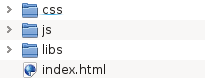
\includegraphics[width=0.4\textwidth]{backbone_structure}
\caption{Структура каталогов}\label{backbone_structure}
\end{figure}

\subsection{Реализация представлений}

Первым делом были написаны шаблоны представлений:

\begin{enumerate}
 \item Представление для создания нового задания. .
 \item Представление для просмотра списка поставленных задач.
 \item Представление для вывода подробной информации об исследовании.
 \item Шаблон для построения графика результата.
\end{enumerate}

Представление для создания нового задания получается довольно динамическим: форма генерируется налету, ее компоненты зависят от выбранного алгоритма, что приводит к перестройке формы при смене алгоритма. В более-менее сложных разметках использование HTML кода внутри JavaScript довольно бессмысленная затея. Код становится запутанным и сложнее для понимания, а также теряются преимущества использования среды разработки. К сожалению, библиотека Backbone.JS не имеет встроенного шаблонизатора --- авторы оставляют выбор за разработчиком. Поэтому был написан свой, основанный на шаблонизаторе Mustache из библиотеки Underscore.js. Его основное отличие в том, что заимствованная библиотека позволяет хранить шаблон только в виде строки, в то время как написанный шаблонизатор из файлов. Шаблон представляет собой скрипт с типом \textbf{text/template} и имеет уникальный идентификатор. Тело шаблона представлено в виде расширенного HTML и компилируется написанной функцией template. В ходе компиляции происходит санитизация полученных данных, интерполяция переменных и необходимые вычисления для чего используется специальный синтаксис <\% ... \%> и <\%= … \%>. Пример кода шаблона отображен на рисунке \ref{template_example}. Скомпилированный шаблон отражен на рисунке \ref{new_issue}.

\begin{figure}[ht]
\center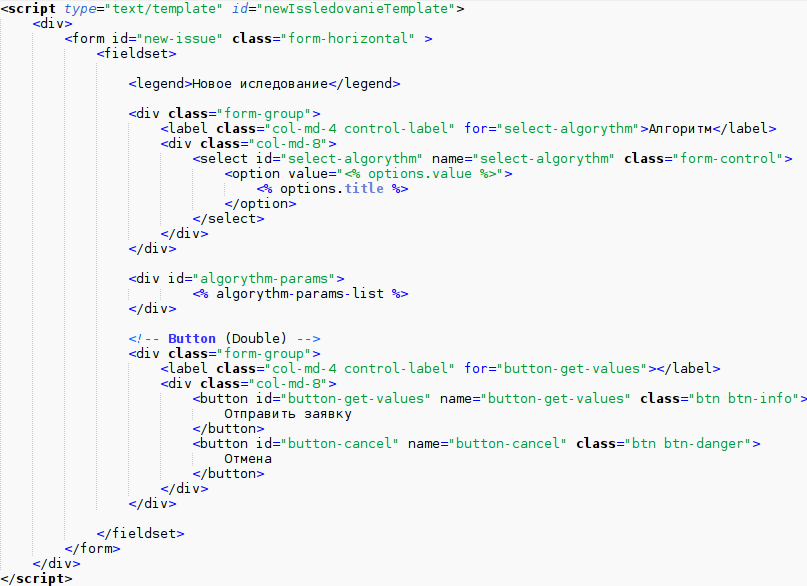
\includegraphics[width=\textwidth]{template_example}
\caption{Пример шаблона}\label{template_example}
\end{figure}

\begin{figure}[ht]
\center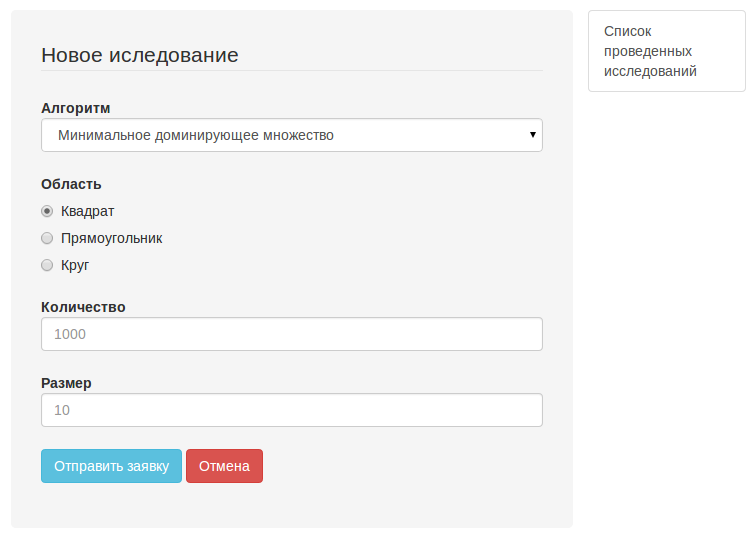
\includegraphics[width=\textwidth]{new_issue}
\caption{Пример шаблона}\label{new_issue}
\end{figure}

Для быстрой разработки и верстки шаблонов в ходе создании представлений активно использовалась библиотека Twitter Bootstrap. Это свободный набор инструментов, включающий в себя CSS шаблоны оформления веб-форм, кнопок, меток, блоков навигации. Он использует самые современные наработки в области CSS и HTML и позволяет сэкономить время и усилия, используя шаблоны дизайна. Также все компоненты платформы Bootstrap используют единый стиль благодаря чему веб-страницы имеют приятный интерфейс.

Представление для просмотра списка поставленных задач не отличается ни чем примечательным: это нумерованный список результатов. Результат отображен на рисунке \ref{list}. Результаты, находящиеся в очереди, обведены серым фоном и недоступны для подробного просмотра. Вывод подробной информации об исследовании аналогичен созданию нового. Если результатом исследования является график, то задействуется специальный шаблон. Он позволяет курсором подробно изучать полученные значения характеристик в различных точках графика. Скомпилированный шаблон отражен на рисунке \ref{result}.

\begin{figure}[ht]
\center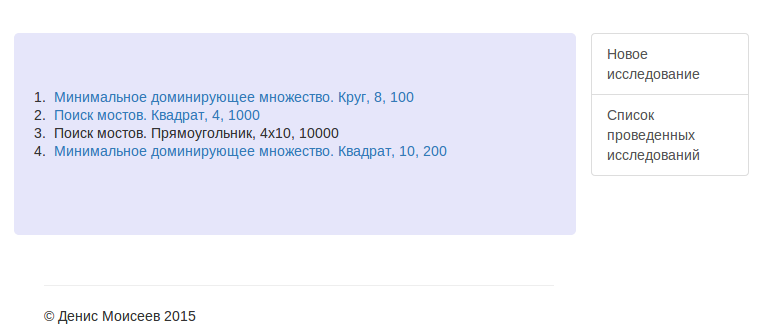
\includegraphics[width=\textwidth]{list}
\caption{Пример шаблона}\label{list}
\end{figure}

\begin{figure}[ht]
\center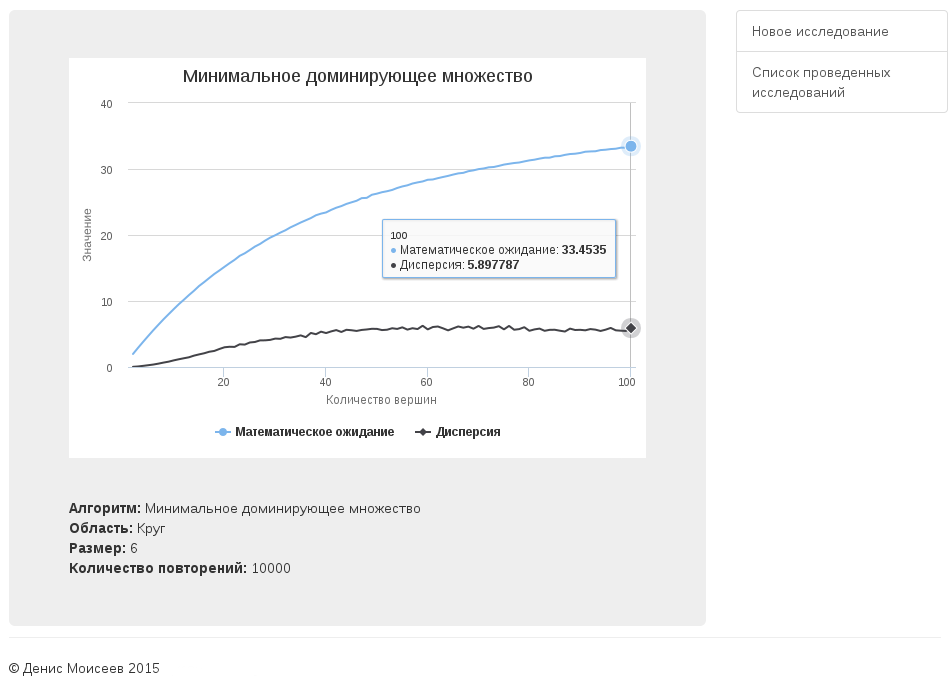
\includegraphics[width=\textwidth]{result}
\caption{Пример шаблона}\label{result}
\end{figure}

\lstset{ %
  language=JavaScript
}

После того как были подготовлены основные шаблоны, можно приступить к созданию вида в Backbone. Для этого достаточно расширить базовый класс, задать базовый тег и переопределить метод render():
\begin{lstlisting}
var IssueListView = Backbone.View.extend({
  tagName: 'ol',
  template: template('listTemplate'),
  render: function() {
    var elem = this.template(this.toJSON());
    this.$el.html(elem);
  }
});
\end{lstlisting}
Исходные коды всех представлений и шаблонов отображены в приложении А.

\subsection{Хранение данных}

Представления созданы, теперь необходимо позаботиться о хранении данных в процессе работы программы. Данные в программах, написанных с использованием Backbone.js хранятся в моделях --- специальных конструкторов объектов с уже готовым набором служебных методов. Создание модели происходит достаточно просто --- необходимо расширить базовую модель:
\begin{lstlisting}
var IssueModel = Backbone.Model.extend({
  defaults: {
    type: null,
    area: null,
    size: 0,
    step_count: 0,
    vertex_count: 0
  }
});
\end{lstlisting}
Таким образом, создается новый класс Model, который принимает параметром анонимный объект и класс модели наполняется значениями. После создания класса модели, для инстанцирования экземпляра класса можно воспользоваться стандартным способом при помощи new, при этом конструктору передается объект с данными, которые попадут в экземпляр класса:
\begin{lstlisting}
var issue = new IssueModel({
  type: "min_dom",
  area: "circle",
  size: 8,
  step_count: 1000,
  vertex_count: 100
});
\end{lstlisting}
Для доступа к атрибутам модели или создания новых в процессе исполнения программы необходимо воспользоваться методами get() и set(). В отличие от прямого доступа к данным, использование getter'ов и setter'ов инкапсулирует доступ к данным экземпляра, а также позволяет контроллерам отреагировать на изменение модели --- произойдет рассылка события 'change' всем подписанным контроллерам на этот экземпляр.

Для описания модели исследования была спроектирована следующая структура модели, отображенная на рисунке \ref{issue_model_backbone}. Самые основные атрибуты, которые присутствуют у большинства исследований (алгоритм, тип исследуемой области, размер области, количество вершин, количество повторений запуска алгоритма и основные статистические характеристики) были вынесены в класс модели. Остальные атрибуты, которые присутствуют только у конкретных алгоритмов могут быть легко добавлены в модель при помощи метода set().

\begin{figure}[ht]
\center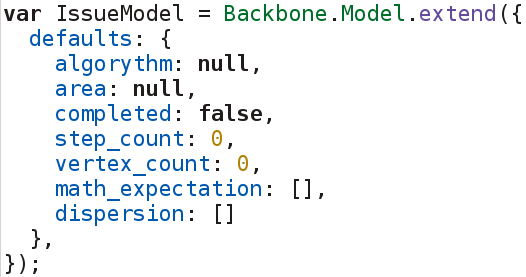
\includegraphics[width=0.75\textwidth]{issue_model_backbone}
\caption{Реализация модели исследования}\label{issue_model_backbone}
\end{figure}

Пока что создана только модель описания исследования. Но в приложении необходимо оперировать не одним объектом. Конечно, можно создать нужное количество экземпляров модели, потом для каждой создать отдельные экземпляры представлений и связать их. Однако, в таком случае код будет захламлен целой кучей экземпляров моделей и представлений. В таком случае, для хранения списка результатов существует удобное решение, встроенное в Backbone --- коллекции.

Коллекции в Backbone.js по сути являются массивами экземпляров моделей. Однако, помимо этого у них есть дополнительный функционал, который делают их вне конкуренции по сравнению с обычными массивами.

Коллекции создаются путем расширения базовой коллекции. Чтобы связать коллекцию с моделью, при ее создании в свойстве model передают ссылку на модель. Например:
\begin{lstlisting}
var IssueCollection = Backbone.Collection.extend({
  model: IssueModel
});
\end{lstlisting}
После этого можно создавать экземпляр коллекции и передавать либо ссылку на существующий экземпляр модели, либо массив с несколькими экземплярами моделей:
\begin{lstlisting}
var issue2 = new IssueModel({
  type: "bridge",
  area: "square",
  size: 4,
  step_count: 500,
  vertex_count: 100
});

var issueCollection = new IssueCollection([issue, issue2]);
\end{lstlisting}
После создания коллекции понадобится возможность создания и удаления моделей из коллекции. Для этого можно воспользоваться методами add() и remove(). Основное преимущество от использования коллекций заключается в том, что при изменении списка результатов произойдет автоматическое обновление представлений благодаря системе событий. Любое событие, которое сработает на модели в коллекции также сработает и напрямую --- для удобства --- на коллекции. Это позволяет напрямую слушать события изменения отдельных атрибутов любой модели в коллекции \cite{backbone}.

\subsection{Реализация логики приложения}

Теперь, когда готовы модель и представления пришло время соединить их контроллерами. Для начала нам необходимо отслеживать текущее состояние приложения. Необходимо определить --- создает ли пользователь новую заявку или же он просматривает список проведенных исследований. А может вообще запрашивает результат.  Конечно эту информацию можно хранить в каких-то внутренних переменных, но обычно попутно нужно решить еще одну задачу — пользователь должен иметь возможность сохранять текущее состояние приложения, чтобы потом вернуться к нему, как будто перерыва во времени и не было вовсе. Часть информации, такая как созданные заявки, их статус и подробная информация о проведении исследования, хранится на сервере, чтобы потом быть загруженной при запуске приложения, а часть, та которая отражает текущее состояние пользовательского интерфейса, обычно хранится в адресной строке браузера. 

Обычно нам необходимо отслеживать изменения в адресной строке, чтобы по-разному реагировать на них, а также иметь возможность самим менять адресную строку, в случае если состояние приложения изменилось. В Backbone есть встроенные средства для легкой реализации подобного поведения.
\begin{enumerate}
\item Роутер (Router). Занимается маршрутизацией. В этот объект записываются все возможные шаблоны (роуты) для адресной строки, а также соответствующая каждому шаблону функция, которая будет вызвана, в случае если текущая адресная строка будет ему удовлетворять\cite{backbone}.

\item История (History). Запускает отслеживание изменений. У объекта Backbone.History есть только один встроенный метод start. Backbone поддерживает отражение текущего состояния в адресной строке как с помощью хэшей (\#issue/108), так и с помощью History API (issue/108) в тех браузерах, которые это поддерживают, деградируя до использования хешей в старых браузерах\cite{backbone}.
\end{enumerate}

Роутер создается путем расширения базового класса Backbone.Router. Все маршруты записываются в виде ассоциативного массива в свойство routes. В паре ключ-значение в ключ записывается шаблон для адресной строки, а в значение --- строка с названием функции, которая будет вызвана в случае совпадения. Сами вызываемые функции записываются в свойства будущего класса роутера:
\begin{lstlisting}
AppRouter = Backbone.Router.extend({
  routes: {
    '': 'list_issues',
    "issue": 'list_issues',
    "issue/new": 'create_issue',
    'issue/:id': 'display_issue',
    '*': 'list_issues'
  },
  list_issues: function() {
    issues.fetch();
    issues_view = new IssueListView({collection: issues});
    content_element.html(issues_view.render());
  },
  display_issue: function(id) {
    issue = issues.get(id);
    content_element.html(template('IssledovaniaTemplate')(issue));
  }
\end{lstlisting}

Каждая такая функция является контроллером в модели проектирования MVC. В данной работе понадобилось написать три таких контроллера: для отображения списка результатов (отображен выше), для создания новой заявки и для отображения конкретного результата исследования. Начнем с реализации контроллера для создания новой заявки. Получим данные об алгоритмах с сервера, заполним шаблон. Также необходимо обработать отправление результата веб-сервису:
\begin{lstlisting}
create_issue: function() {
  var data = algorythms.fetch();
  content_element.html(template('newIssledovanieTemplate')({
    options: data,
    algorythm_params_list: function() {data.render()}
  }));
  $('#submit').submit( function( e ) {
    var data = $(this).serializeArray();
    var issue = new IssueModel(data);
    issue.save();
    issue.once("sync", function(issue){
      issues.add(issue);
    });
    location.href = "#";
    e.preventDefault();
  });
},
\end{lstlisting}
Данный код отображен схематически, полная реализация контроллеров доступна в приложении Б. Контроллер для отображения результата не особым не отличается и также был отображен выше.

\section{Создание приложения с использованием AngularJS}

После использования фреймворка Backbone.js было решено реализовать приложение с использование с целью выяснения практических преимуществ и недостатков.

Первым делом было решено автоматизировать развертывание приложения и воспользоваться такими средствами как npm и Bower. Npm --- это пакетный менеджер для JavaScript, который является частью проекта Node.js. Этот инструмент позволяет автоматизировать сборку приложения (с использование Bower), тестирование и развертывание. Установка не отличается ничем примечательным --- необходимо из репозиториев или же с официального сайта (http://nodejs.org) произвести установку Node.js и npm идет с ним же\cite{npm}. Все инструкции для автоматизации находятся в файле package.json. В процессе реализации данного приложения был написан следующий файл конфигурации:
\begin{lstlisting}
{
  "name": "adhoc-project",
  "devDependencies": {
    "http-server": "^0.6.1",
    "bower": "^1.3.1"
  },
  "scripts": {
    "postinstall": "bower install",
    "prestart": "npm install",
    "start": "http-server -a 0.0.0.0 -p 8080"
  }
}
\end{lstlisting}

Такая конфигурация позволяет из командой строки выполнить:
\begin{lstlisting}
npm run
\end{lstlisting}

И произойдет следующее: установятся все необходимые зависимости для развертывания приложения, выполнится bower install и запустится веб-сервер на 8080 порту. Таким, образом, не нужно включать в проект зависимые библиотеки --- это произойдет автоматически, основываясь на конфигурации, описанной в package.json.

Для управления зависимостями JavaScript-библиотек был выбран менеджер пакетов Bower. Bower --- не стандартный менеджер пакетов, но самый популярный. Сейчас в репозитории находится более 11 тысяч пакетов\cite{bower}. Bower не навязывает пользователю свою систему сборки, а разработчику пакетов --- метод подключения библиотеки. Всё, что делает Bower --- устанавливает нужные проекту пакеты подходящих версий вместе с их зависимостями. Другими словами: просто загружает файлы нужных библиотек и всё, что нужно для их работы в специальную папку. Остальное остается на усмотрение разработчика.

После установки и настройки npm необходимо настроить конфигурацию Bower. Для этого в каталог проекта необходимо добавить файл bower.json, с содержимым которые напоминает конфигурацию npm:
\begin{lstlisting}
{
  "name": "adhoc-project",
  "private": true,
  "dependencies": {
    "jquery": "",
    "easysoap": "",
    "bootstrap": "3.3.4",
    "angular": "~1.4.0",
    "angular-route": "~1.4.0",
    "angular-resource": "~1.4.0"
  }
}
\end{lstlisting}

% \subsection{Структура приложения}
% 
В процессе реализации данного приложения была создана следующая структура каталогов, отображенная на рисунке \ref{angular_structure}. В каталогах \textit{bower\_components} и \textit{node\_modules} хранятся библиотеки, от которых зависит данный проект. Они обновляются автоматически при помощи утилит npm и bower.
\begin{figure}[h]
\center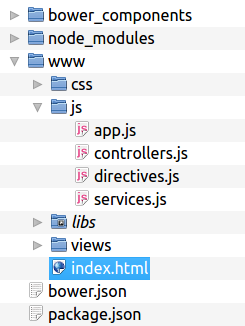
\includegraphics[width=0.4\textwidth]{angular_structure}
\caption{Структура каталогов приложения на AngularJS}\label{angular_structure}
\end{figure}

В каталоге \textit{www} хранится само приложение, где \textit{index.html} --- точка входа приложения. В каталоге \textit{css} находятся таблицы стилей, в каталоге \textit{views} шаблоны представлений. Каталог \textit{libs} представляет собой символическую ссылку на каталог bower\_components и содержит в себе необходимые проекту библиотеки.

При реализации данного проекта потребовались следующие библиотеки:
\begin{enumerate}
 \item jQuery. Библиотека JavaScript, фокусирующаяся на взаимодействии JavaScript и HTML\cite{jquery}.
 \item easySoap. WSDL SOAP клиент для JavaScript.
 \item Twitter Bootstrap. Свободный набор инструментов для создания сайтов и приложений. Включает в себя HTML и CSS шаблоны оформления\cite{bootstrap}.
 \item AngularJS. JavaScript-фреймворк предназначенный для разработки одностраничных приложений на основе MVC шаблона\cite{angular}.
\end{enumerate}

В каталоге \textit{js} находятся четыре JavaScript-скрипта, логически разделенные на различные части приложения: маршрутизация, контроллеры, директивы, сервисы:
\begin{enumerate}
 \item app.js. Описывается структура приложения: используемые модули и маршрутизация.
 \item controllers.js. Модуль, который содержит в себе все контроллеры, определенные в данном проекте.
 \item directives.js. Модуль с реализованными дополнительными директивами: для построения графика и для вывода сообщений.
 \item services.js. Модуль, в котором реализованы различные сервисы для работы с данными: получение/отправка данных на сервис по протоколу SOAP, сервис для обработки сообщений пользователю и сервис для перевода машинных идентификаторов в формат, понятный человеку.
\end{enumerate}

\subsection{Точка входа, шаблоны и представления}

Точкой входа в одностраничное приложение является файл \textit{index.html}. Это HTML страница, которая строится при помощи HTML приведенного ниже. Данный код также содержит некоторые ключевые angular директивы.
\begin{lstlisting}[basicstyle=\footnotesize]
<!doctype <!DOCTYPE html>
<html ng-app="adhocApp">
<head>
  <meta charset="utf-8">
  <title>Вероятностная система в модели AD-HOC сети</title>
  <link rel="stylesheet" href="libs/bootstrap/dist/css/bootstrap.min.css">
  <link rel="stylesheet" href="css/style.css">

  <script src="libs/jquery/dist/jquery.min.js"></script>
  <script src="libs/easysoap/easysoap.js"></script>
  <script src="libs/angular/angular.min.js"></script>
  <script src="libs/angular-route/angular-route.min.js"></script>
  <script src="libs/angular-resource/angular-resource.min.js"></script>
</head>
<body>

 <div class="container">
    <div class="row row-offcanvas row-offcanvas-right">
      <div class="col-xs-12 col-sm-9" id="content">
        <div ng-view></div>
      </div>

      <div class="col-xs-6 col-sm-3 sidebar-offcanvas" id="sidebar" role="navigation">
        <div class="list-group">
          <a href="#new" class="list-group-item">Новое исследование</a>
          <a href="#issue" class="list-group-item">Список проведенных исследований</a>
        </div>
      </div>
    </div>
</div>

<script src="js/app.js"></script>
<script src="js/controllers.js"></script>
<script src="js/services.js"></script>
<script src="js/directives.js"></script>
</body>
</html> 
\end{lstlisting}
Директива ng-app используется как флаг, который сообщает Angular-у корневой элемент нашего приложения. Это позволяет определить всю HTML-страницу как Angular-приложение. При загрузке приложения происходит автоматическая инициализация при помощи директивы ngApp.

В разделе \textit{head} определены сторонние библиотеки, без которых невозможна работа данного приложения. В разделе \textit{body} описывается основная структура приложения с использованием Twitter Bootstrap. Создается колоночный макет, состоящий из двух колонок: содержимое страницы и навигация.

Отображение содержимого страницы происходит при помощи директивы ngView. После этапа инициализации приложения, Angular создаёт инжектор, который будет использован во всем приложении, подгружаются необходимые зависимости, и происходит компиляция DOM. И директива ngView позволяет включать в себя шаблон текущего представления. Это возможно потому, что Angular поддерживает частичные представления и это позволяет отлично отделять логику от представления.

HTML отлично подходит для описания статичных документов, но теряет свою эффективность при попытке описать динамические виды в веб-приложениях. AngularJS позволяет расширить синтаксис HTML. В результате код получается выразительным, читаемым, и легко поддерживается.

Другие фреймворки обходят недостатки HTML либо абстрагируясь от HTML, CSS или JavaScript, либо навязывая обязательные инструменты для манипулирования DOM. Ни один из этих способов ни устраняет суть проблемы, а именно то, что HTML не предназначен для динамических приложений.

В Angular'е, представление (view) это проекция модели (model) через HTML-шаблон (template). Это означает, что всякий раз, когда модель изменяется, Angular обновляет соответствующие связывания (binding points), которые обновляют представление (view). Представление (view) строится Angular`ом из шаблона. Шаблоны для данного проекта помещены в каталог \textit{views} и подгружаются при необходимости. Шаблоны использовались те же, что и в приложении на Backbone.js и были адаптированы специально под AngularJS. Вместо шаблонизатора использовались определенные директивы, но сам стиль приложения остался тот же. Исходные коды шаблонов представлены в приложении А.

\subsection{Маршрутизация и контроллеры}

Все приложения в AngularJS создаются через модули. Модуль может зависеть от других, или быть одиночным. Модули служат контейнерами для разных разделов приложения, таким образом делая код пригодным для повторного использования. Для создания модуля применяется глобальный Object, пространство имен фреймворка, и метод module:
\begin{lstlisting}
var adhocApp = angular.module('adhocApp', [
  'ngRoute',
  'adhocControllers',
  'adhocServices',
  'adhocDirectives'
]);
\end{lstlisting}

Первым параметром указывается название модуля, вторым аргументом идет список зависимостей модуля, которые также нужно подключить. Модули могут зависеть от других модулей, которые в свою очередь тоже могут иметь зависимости.
Инициализация AngularJS приложения происходит автоматически, используя директиву ngApp. Затем инициализируется Инжектор, который будет использоваться для внедрения зависимости (dependency injection) в рамках создания приложения. Инжектор будет создавать корневую область видимости (root scope), которая станет контекстом для модели нашего приложения. Angular будет"компилировать DOM, начиная с корневого элемента ngApp, подготавливая найденные директивы и связывая директивы с соответствующими элементами\cite{angular:tutorial}.

Маршруты в Angular задаются с помощью \$routeProvider'а, который предоставляет сервис \$route. Этот сервис позволяет легко связывать воедино контроллеры, шаблоны представления и текущий URL браузера:
\begin{lstlisting}
$routeProvider.
  when('/issue', {
    templateUrl: 'views/issue-list.html',
    controller: 'IssueListController'
  }).
  when('/new', {
    templateUrl: 'views/new-issue.html',
    controller: 'AlgorithmController'
  }).
  when('/issue/:id', {
    templateUrl: 'views/result.html',
    controller: 'ResultController'
  }).
  otherwise({
    redirectTo: '/issue'
  });
\end{lstlisting}

Контроллер Angular сводит вместе бизнес-логику и логику представления. Контроллер принимает два аргумента – имя, по которому на него можно ссылаться, и функцию описывающее поведение контроллера:
\begin{lstlisting}
angular
  .module('adhocControllers', [])
  .controller('IssueListController', ['$scope', 'Results', IssueListController]);

function IssueListController($scope, Results) {
  Results.query()
    .$promise.then(function (result) {
      angular.forEach(result, function(index) {
        var name = index.algorithm + '. ';
        name += index.area + ', ';
        name += '' + index.size + ', ' + index.step;
        index.name = name;
      });
      $scope.issues = result;
  });
}
\end{lstlisting}

Контроллер общается с Сервисом, и передает данные в том же, или измененном формате в наш Вид через объект \$scope. Когда Вид обновлён, логика Контроллера также обновляется, и её можно передавать обратно на сервер через Сервис. Благодаря двухстороннему связыванию, любые изменения, внесенные в модель отражаются в представлении, любые изменения, которые происходят в представлении отражаются в модели. Остальные контроллеры идентичны контроллерам в Backbone.js и были адаптированы под использование в AngularJS. Исходные коды отображены в приложении В.




\section{Создание мобильного приложения}

В рамках данной аттестационной работы было разработано кроссплатформенное мобильное приложение системы вероятностного моделирования с использованием фреймворка Apache Cordova. Данное приложение можно скомпилировать на множество платформ, поддерживаемых Apache Cordova, в частности это: Tizen, webOS, Android, iOS, Blackberry, Samsung Bada и Windows Phone. Тестировалось приложение на платформе Android 4.0.4 Ice Cream Sandwich.

\subsection{Настройка окружения}
Перед началом процесса разработки мобильного приложения необходимо настроить окружение, установить необходимые библиотеки и средства разработки. Для начала, необходимо убедиться, что NodeJS уже установлен и доступен для использования:
\begin{lstlisting}
 $ nodejs --version
 $ npm --version
\end{lstlisting}

Обе команды необходимо выполнить в командной строке и убедиться в том, что они успешно выполнились. В противном случае необходимо установить необходимые программы. Далее, установим необходимые библиотеки и их зависимости:
\begin{lstlisting}
 $ npm install -g cordova
\end{lstlisting}

Данная команда скачает из репозитория npm файл package.json для проекта cordova, создаст файлы, относящиеся к проекту, установит все зависимости, необходимые для корректной работы данного фреймворка, а также создаст ссылки на исполняемые файлы. Результат работы этой команды отображен на рисунке \ref{npm_cordova}. После завершения скрипта в нашей системе появится возможность использовать Cordova CLI из любого места за счет глобальной пролинковки (атрибут -g в команде установки).

\begin{figure}[ht]
\center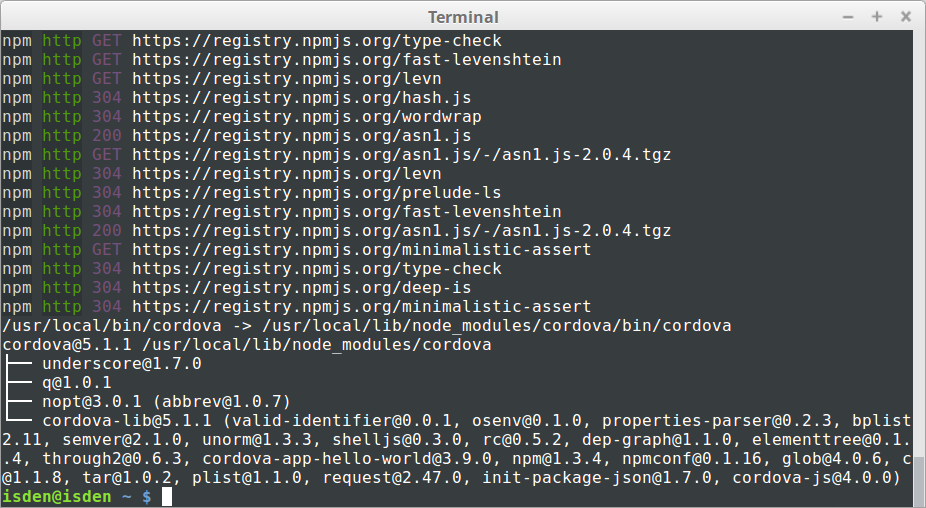
\includegraphics[width=0.9\textwidth]{npm_cordova}
\caption{Результат установки cordova}\label{npm_cordova}
\end{figure}

Для сборки проекта под Android необходимо установить и настроить Java SDK и Android SDK. Для этого скачиваем последние версии наборов разработки с официального сайта Oracle\cite{cordova:java_sdk} и официального сайта Google\cite{cordova:android_sdk}. Установка Java SDK не отличается ничем примечательным. После установки необходимо убедиться что правильно задана переменная окружения JAVA\_HOME.

Установка Android SDK отличается на различных платформах. Например, под ОС Windows необходимо запустить инсталлятор и следовать полученным инструкциям от мастера установки. Под ОС GNU$\backslash$Linux дистрибутив распространяется в качестве простого архива, который достаточно просто распаковать. После установки запускаем утилиту настройки \textit{android}, которая находится в каталоге tools. Для сборки проекта в Apache Cordova необходимы Build Tools последних версии, а также Platform Tools и Tools. Также необходимо установить SDK Platform версии не ниже 22. Пометим флажками для установки нужные компоненты (рисунок \ref{android_sdk}), прочтем лицензионное соглашение и ожидаем окончания процесса скачивания и установки. После проведения данных манипуляций, необходимо убедиться в том, задана переменная ANDROID\_HOME, которая указывает расположение Android SDK. что в переменной PATH добавлен путь к каталогам tools и platform-tools. Теперь все готово для начала процесса разработки.
\begin{figure}[ht]
\center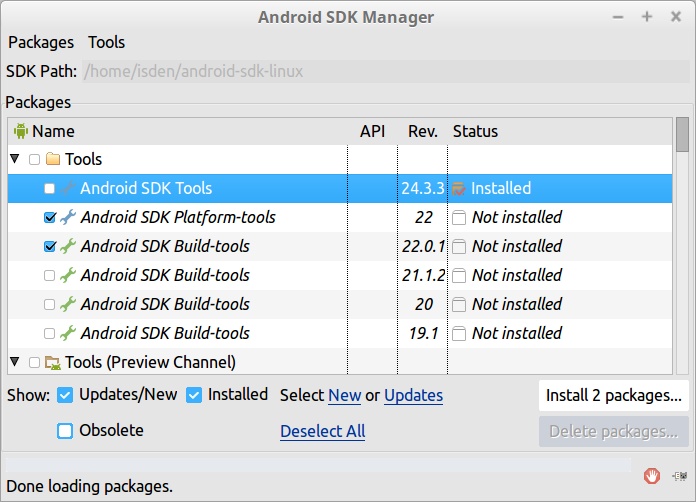
\includegraphics[width=0.9\textwidth]{android_sdk}
\caption{Окно настройки средств разработки Android}\label{android_sdk}
\end{figure}

\subsection{Адаптация приложения}
Для начала работ по переносу веб-приложения на мобильные устройства необходимо создать базовую структуру каталогов. Для этого воспользуемся командой:
\begin{lstlisting}
 $ cordova create adhoc-system
 $ cordova platform add android
\end{lstlisting}

Первая команда создаст необходимые для работы каталоги и файлы конфигурации. Структура каталогов отображена на рисунке \ref{cordova_structure}. Директория \textit{platforms} включает в себя раздельный код под каждую из используемых платформ. Компилируется каждый раз при выполнении сборки. В директории \textit{plugins} находятся подключаемые библиотеки Cordova, используемые в приложении. Например для работы с консолью вывода устройства. Каталог www представляет собой наше веб-приложение. Также в корне проекта есть файл \textit{config.xml}, отвечающий за основные настройки приложения. Этот файл является самой важной частью проекта на основе Apache Cordova. Он включает в себя ссылки на ресурсы приложения, устанавливает необходимые разрешения и настраивает параметры для каждой из платформ (например поведение статусной строки). Идентификатор приложения (bundle) и информация об издателе должна быть также указана в файле \textit{config.xml}.
\begin{figure}[ht]
\center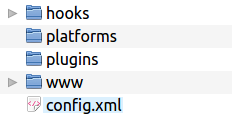
\includegraphics[width=0.5\textwidth]{cordova_structure}
\caption{Структура проекта Apache Cordova}\label{cordova_structure}
\end{figure}

Плагины в Apache Cordova представляют собой пакеты, которые позволяют внедрить нативный код в приложение и управлять методами из Cordova Web View. Все основные функции Cordova API реализованы при помощи плагинов, которые предоставляют доступ к возможностям и функциям устройства и платформы, которые недоступны обычному веб-приложению: например доступ к камере, NFC, уведомления в в статусной строке и даже доступ к отпечаткам пальцев, при наличии данной возможности в аппарате\cite{android:publish}. В данной работе плагин не был реализован, хватило встроенных возможностей Cordova API.

Существует отдельный репозиторий Cordova плагинов. Все плагины обычно имеют документацию и примеры использования, а также содержат исходный код на GitHub. Для отладки был подключен плагин cordova-plugin-console, который позволяет дублировать вывод команды console.log в лог отладки приложения, доступный средствами отладки конкретной платформы. Его установка производится следующей инструкцией:
\begin{lstlisting}
 cordova plugin add cordova-plugin-console
\end{lstlisting}

После всех приготовлений можно переносить код написанного с использованием AngularJS приложения в каталог www. Так как сборка будет производиться без использования bower, то вручную предварительно выполним команду \textit{bower install}. 

Для мобильных телефонов, имеющих низкое разрешение экрана, с целью компактно разместить компоненты на экране, были написаны новые таблицы стилей. Для этого был продуман и создан отдельный дизайн веб-страниц. Этот дизайн обеспечивает корректное отображение представлений приложения на различных устройствах, запускающих мобильное приложение и динамически подстраивающийся под заданные размеры экрана аппарата. Таким образом, приложение удобно просматривается с устройств различных разрешений и форматов. Теперь не нужно реализовывать отдельные версии представлений для отдельных видов устройств. Одно представление может работать как на устаревших аппаратах, так и на современных экранах, обладающих высокой плотностью пикселей. Такой подход практикуют большинство современных разработчиков мобильных приложений и веб-мастеров. Пример стиля для адаптивного дизайна отображен ниже:
\begin{lstlisting}
  #sidebar {
    position: absolute;
    right: 0;
  }

  @media screen and (max-width: 700px) {
    #sidebar {
      position: fixed;
      bottom: 0;
      right: auto;
      width: 100%;
    }
    #sidebar a {
      float: left;
    }
    body {
      padding-bottom: 100px;
    }
  }
\end{lstlisting}

После создания проекта и проведенной адаптации приложения к мобильному виду, все готово для сборки приложения под различные платформы.

\subsection{Сборка приложения}

Сборку приложения будем производить на примере Android, под другие платформы действия аналогичны. Сборка максимально автоматизирована при помощи такого средства сборки как Gradle. Gradle пытается объединить в себе все плюсы Ant, Maven и Ivy. И представить то, что получилось, с помощью Groovy. Теперь вместо того, чтобы скрещивать Batch-скрипты, java и xml-файлы конфигурации, можно просто написать несколько строчек кода на диалекте Groovy. Диалект специально разработан для описания сборки, тестирования, развертывания, экспорта и других действий над проектом. Также присутствует следующая возможность: соответствующим образом настроенный Gradle-проект можно собрать на машине пользователя, на которой Gradle не установлен. Все, что требуется, --- положить в дерево исходников 4 файла (которые Gradle сгенерирует автоматически): 2 исполняемых для Win/*nix, 1 файл настроек и маленький jar. Всего на 20Kb. После этого проект можно собрать на любой машине, где есть доступ к Интернет. Скрипт сам позаботится о скачивании правильной версии Gradle, о настройке и запуске сборки\cite{android:publish}.

Apache Cordova настраивает проект как раз таким образом. Поэтому для сборки debug-версии необходимо воспользоваться следующей командой:
\begin{lstlisting}
  cordova build android
\end{lstlisting}
Процесс сборки отображен на рисунке \ref{cordova_build}. Сборка релизной версии осуществляется командой:
\begin{lstlisting}
  cordova build --release android
\end{lstlisting}
\begin{figure}[ht]
\center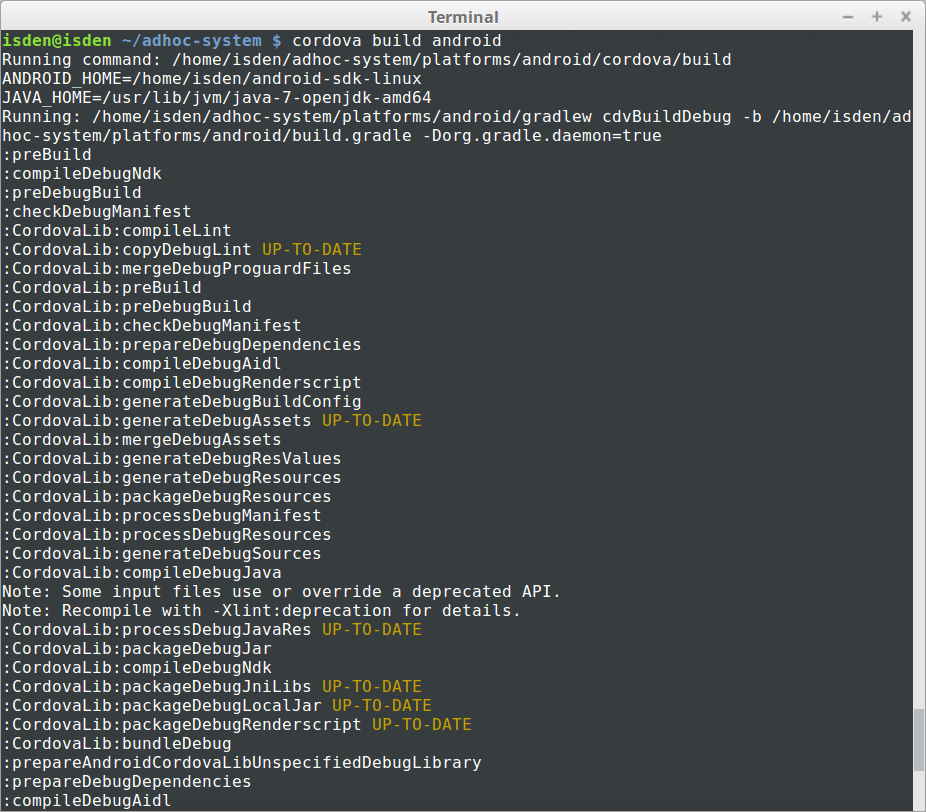
\includegraphics[width=0.7\textwidth]{cordova_build}
\caption{Сборка проекта Apache Cordova}\label{cordova_build}
\end{figure}

Таким образом сгенерирован неподписанный .apk файл, который будет находиться в каталоге \textit{platforms/android/build/outputs/apk}. Теперь необходимо подписать неподписанное приложение, для этого необходимо сгенерировать ключ с помощью утилиты keytool, которая уже включена в состав Android SDK.

Далее, необходимо выполнить в командной строке следующую команду: 
\begin{lstlisting}
keytool -genkey -v -keystore my-release-key.keystore -alias alias_name -keyalg RSA -keysize 2048 -validity 10000.
\end{lstlisting}
В процессе выполнения которой потребуется ввести пароль для keystore, по умолчанию пароль --- \textit{android}. Затем требуется ввести ответы на ключевые вопросы вроде: ФИО, организация, город, регион, страна. Далее подтверждаем введённые данные и вводим пароль для ключа, по умолчанию он androiddebugkey\cite{android:publish}.

Ключ готов, теперь необходимо подписать этим ключом приложение, для этого необходимо поместить неподписанное приложение в ту же папку где и ключ, затем выполнить подписание при помощи утилиты \textit{jarsigner}. Для этого необходимо выполнить следующую команду: 
\begin{lstlisting}
jarsigner -verbose -sigalg SHA1withRSA -digestalg SHA1 -keystore my-release-key.keystore android-release-unsigned.apk alias_name
\end{lstlisting}

Теперь приложение подписано и готово к установке на устройство Android. Файл приложения копируем на устройство и для установки необходимо в настройках устройства отметить разрешение установки приложений из неизвестных источников.

Скриншот работающего приложения на моём устройстве представлен на рисунке \ref{cordova_runned}.
\begin{figure}[ht]
\center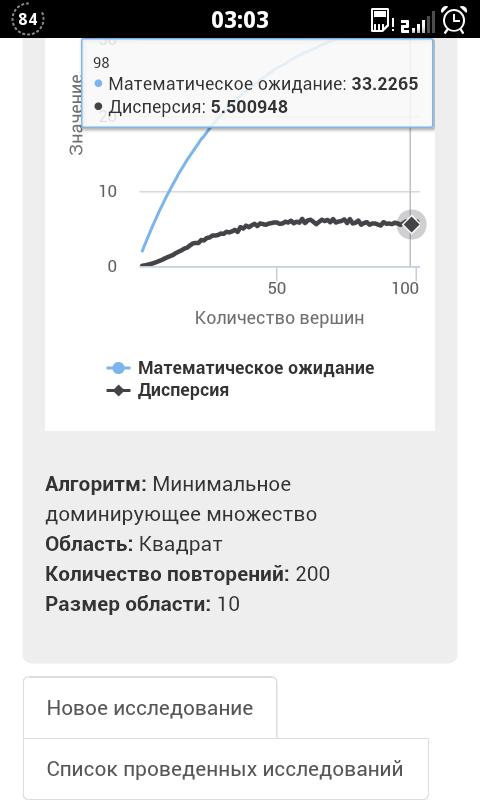
\includegraphics[width=0.45\textwidth]{cordova_runned}
\caption{Запущенное приложение}\label{cordova_runned}
\end{figure}

\frontmatter{Заключение}

В рамках данной выпускной квалификационной работы бакалавра были рассмотрены основные способы создания эффективных и удобных веб-приложений с использованием шаблонов проектирования. Также были изучены преимущества и недостатки различных инструментов как с теоритической так и с практической стороны.

Пользуясь полученными знаниями, было разработано кроссплатформенное приложение для системы вероятностного моделирования ad-hoc сетей с использованием AngularJS. Далее, это приложение было развернуто для запуска на широком спектре мобильных устройств с использованием Apache Cordova. Был использован SOAP сервис для обмена данными.

\begin{thebibliography}{30}
\bibitem{cordova:android_sdk} Download Android Studio and SDK Tools. [Электронный ресурс], Android Developers, URL: https://developer.android.com/intl/ru/sdk/index.html, [Дата обращения: 6 июня 2015].

\bibitem{cordova:java_sdk} Java SE - Downloads. [Электронный ресурс], Oracle Technology Network, URL: http://www.oracle.com/technetwork/java/javase/downloads/index.html, [Дата обращения: 6 июня 2015].

\bibitem{mobile_count} Список стран по числу используемых мобильных телефонов. [Электронный ресурс], Электронная энциклопедия Wikipedia, URL: https://ru.wikipedia.org/wiki/Список\_стран\_по\_числу\_используемых\_моби- льных\_телефонов, [Дата обращения: 13 мая 2015].

\bibitem{cordova} Apache Cordova – фреймворк для создания мобильных приложений [Электронный ресурс], Официальный сайт Apache Cordova, URL: http://cordova.apache.org, [Дата обращения: 13 мая 2015].

% \bibitem{QA2} Cooper R., Ruger S. A Simple Question Answering System. New York, 2007.
% \bibitem{QA} Gaizauskas R., Humphreys K. A Combined IR/NLP Approach to Question Answering Against Large Text Collection. Sheffield, 2010.
% \bibitem{16} Gruber T. R. A translation approach to portable ontologies. USA, 1993.
% \bibitem{QAS} Guda V., Sanamrudi S. K. Approaches for question answering. International Journal of Engineering Science and technology, 2011-3
% \bibitem{18} Авдошин С.М., Шатилов М.П. Информационные технологии онтологического инжиниринга. M, 2008
\bibitem{web1} Акимов С.В. Технологии Internet. // СПб, 2005
% \bibitem{17} Гладун А.Я., Рогушина Ю.В. Онтологии в корпоративных системах. Оренбург, 2006
% \bibitem{frame} Горбунов-Посадов М. М. Расширяемые программы. М, 1999
\bibitem{VBS} Грошев А.С. программирование на VBS. // М, 2007
\bibitem{perl} Маслов В.В. Введение в Perl. // Оренбург, 2000
% \bibitem{19} Овдей О.М., Проскудина Г.Ю. Обзор инструментов инженерии онтологий. М, 2007
\bibitem{php} Томпсон Л., Веллинг Л. Разработка Web-приложений на PHP и MySQL. // Спб, 2008
% \bibitem{web2} Храмцов П.Б., Брик С.А., Русак А.М., Сурин А.И. Основы web-технологий. М, 2008
% \bibitem{QA1} Hirschman L., Gaizauskas R. Natural language question answering: view from here. USA, 2001
% \bibitem{DB} DBpedia Mappings Wiki URL: http://mappings.dbpedia.org/index.php (дата обращения: 11.05.2015)
% \bibitem{start} START: Natural Language Question Answering System  URL: http://start.csail.mit.edu/index.php (дата обращения: 13.05.2015)
% \bibitem{python} Разработка сайтов и приложений на Python URL: http://secl.com.ua/python.html (дата обращения: 13.05.2015)
% \bibitem{ask} Семантическая поисковая система AskNet URL: http://asknet.ru (дата обращения: 12.05.2015)
% \bibitem{ephyra} Open Source Question Answering Frameworks URL: http://www.ephyra.info/ (дата обращения: 13.05.2015)
% \bibitem{py_fram} WebFrameworks URL: https://wiki.python.org/moin/WebFrameworks (дата обращения: 13.05.2015)
% \bibitem{watson} What is Watson? 
% 
% URL: http://www.ibm.com/smarterplanet/us/en/ibmwatson/what-is-watson.html (дата обращения: 13.05.2015)
% \bibitem{dbpedia} DBpedia  URL: http://dbpedia.org/About (дата обращения: 11.05.2015)
% \bibitem{WA} WolframAlpha. Computation Knowledge Engine URL: http://www.wolframalpha.com/ (дата обращения: 13.05.2015)
% 
% URL: http://www.w3.org/blog/SW/2008/01/15/sparql\_is\_a\_recommendation/ (дата обращения: 12.05.2015)
% \bibitem{SP1} SPARQL Query Language for RDF URL: http://www.w3.org/TR/rdf-sparql-query/ (дата обращения: 13.05.2015)
% 
\end{thebibliography}
% \clearpage
% \bibliographystyle{unsrt}
% \bibliography{bibs}{}

\backmatter{Приложение А}{Код шаблонов и представлений}

\lstset{ %
  language=HTML,
  basicstyle=\scriptsize
}
\centerline{Шаблон формы создания новой заявки}
\lstinputlisting[language=HTML, label=lst:form]{src/form.html}

\centerline{Шаблон списка заявок}
\lstinputlisting[language=HTML, label=lst:list]{src/list.html}

\centerline{Шаблон просмотра результата}
\lstinputlisting[language=HTML, label=lst:result]{src/result.html}

\end{document}
